\chapter{Hasil dan Pembahasan}\label{ch:result}

Bab ini menyajikan hasil dan pembahasan pelaksanaan penelitian, yang dimulai dari pembersihan data, \textit{exploratory data analysis}, pra-pra-pemrosesan data, pelatihan model, hingga optimasi hiperparameter menggunakan Algoritma Genetika. Seluruh hasil eksperimen dievaluasi menggunakan metrik WMAPE, MAE, dan $R^2$, serta dibandingkan dengan model tanpa optimasi dan menggunakan optimasi.

\section{Data Transaksi Pendapatan SMS Internasional}\label{sec:data}

    Data yang digunakan dalam penelitian ini merupakan data dari Perusahaan X, salah satu perusahaan telekomunikasi di Indonesia yang bergerak di bidang \textit{traffic management} SMS internasional. Nama perusahaan disamarkan sesuai perjanjian kerahasiaan data. Seluruh nilai yang mengandung identitas perusahaan tertentu juga telah disamarkan. Data dalam penelitian ini memiliki 19 kolom dan memiliki berbagai tipe atribut dengan keterangan di setiap kolomnya. Deskripsi setiap atribut ditunjukkan pada Tabel 4.1.

    \begin{longtable}{lll}
    \caption{Deskripsi Data Pendapatan SMS Internasional} \\
    \toprule
    \textbf{Fitur} & \textbf{Tipe Data} & \textbf{Keterangan} \\
    \midrule
    \endfirsthead
    
    \toprule
    \textbf{Fitur} & \textbf{Tipe Data} & \textbf{Keterangan} \\
    \midrule
    \endhead
    
    Year & Integer & Tahun transaksi \\
    Month & Integer & Bulan transaksi \\
    Client & String & Nama klien \\
    Client Connection & String & Koneksi klien \\
    Supplier & String & Nama Supplier \\
    Supplier Connection & String & Koneksi supplier \\
    Supplier Connection Link & String & Link koneksi supplier \\
    Route & String & Rute pengiriman \\
    Country & String & Negara \\
    Network & String & Jaringan distribusi \\
    OAProfiled Category & String & Kategori profil OA (\textit{Provider}) \\
    Cost Currency & Integer & Biaya dalam mata uang tertentu \\
    Price Currency & Integer & Harga dalam mata uang tertentu \\
    Profit Currency & Integer & Profit dalam mata uang tertentu \\
    Base Currency & Integer & Mata uang dasar \\
    Total Cost & Integer & Total biaya \\
    Total Sent Messages & Integer & Total pesan terkirim \\
    Total Delivered Messages & Integer & Total pesan berhasil terkirim \\
    \textbf{Total Revenue} & \textbf{Integer} & \textbf{Variabel target penelitian} \\
    \bottomrule
    \end{longtable}
    
\section{Pembersihan Data (\textit{Data Cleaning})}
\label{sec:prapra-pemrosesan_data}

Tahap pembersihan data dilakukan untuk memastikan data trafik SMS internasional periode 2023--2024 berada pada kondisi yang layak analisis, bersih, dan siap untuk proses pemodelan. Tahap pembersihan data terdiri dari normalisasi data, penyamaran data sensitif, pengurutan data berdasarkan waktu, penghapusan kolom yang tidak relevan, dan pembersihan nilai tidak valid.

% \begin{figure}[htbp]
% \centering
% \includegraphics[width=0.92\textwidth]{tugas-akhir/assets/images/prapra-pemrosesan_data.png}
% \caption{Tahapan Prapra-pemrosesan Data}
% \label{fig:alur_prapra-pemrosesan}
% \end{figure}

% ---------------------------------------------------------
\subsection{Normalisasi Data}
\label{subsubsec:normalisasi}

Sebelum dilakukan analisis lanjutan, dilakukan proses normalisasi nilai-nilai kategorik yang terdapat dalam dataset. Dari seluruh kolom yang dianalisis, ditemukan kesalahan pengetikan pada kolom \texttt{Network}. Pada kolom ini ditemukan sebanyak 27 data terdapat nilai "\texttt{Telkomcel}" yang secara semantik merupakan kesalahan ejaan dari "\texttt{Telkomsel}". Tanpa koreksi, inkonsistensi ini berpotensi menyebabkan model memperlakukan kedua nilai tersebut sebagai dua entitas yang berbeda, sehingga merusak representasi distribusi data jaringan (\texttt{Network}) sebenarnya. Oleh karena itu, dilakukan proses normalisasi dengan langkah-langkah berikut:

\begin{enumerate}
    \item Seluruh nilai pada kolom \texttt{Network} dikonversi ke tipe string dan dilakukan penghapusan spasi di awal dan akhir  untuk menghindari kesalahan pencocokan akibat karakter tersembunyi.
    \item Penggantian nilai dilakukan menggunakan ekspresi reguler yang bersifat \textit{case-insensitive}, sehingga semua varian ejaan "\textit{Telkomcel}" maupun "\textit{Telkomsel}" distandarisasi menjadi "\texttt{Telkomsel}".
\end{enumerate}

Hasil normalisasi ditunjukkan pada Tabel \ref{tab:network_normalisasi}. Setelah proses ini, kolom \texttt{Network} hanya memuat satu nilai "\texttt{Telkomsel}" yang sebelumnya tercatat dalam dua bentuk.

\begin{table}[h!]
\centering
\caption{Distribusi nilai kolom \texttt{Network} sebelum dan sesudah normalisasi}
\label{tab:network_normalisasi}
\begin{tabular}{lcc}
\toprule
\textbf{Nilai} & \textbf{Sebelum Normalisasi} & \textbf{Sesudah Normalisasi} \\
\midrule
Telkomsel  & 78.991 & 79.018 \\
Telkomcel  & 27     & 0      \\
\midrule
\textbf{Total} & \textbf{79.018} & \textbf{79.018} \\
\bottomrule
\end{tabular}
\end{table}



% ---------------------------------------------------------
\subsection{Penyamaran Data untuk Privasi}
\label{subsubsec:data_masking}

Dataset \texttt{SMS International.csv} mengandung sejumlah kolom yang memuat informasi identitas bisnis yang bersifat rahasia, seperti nama klien, pemasok, koneksi pemasok, rute trafik, dan jaringan operator. Penggunaan nilai-nilai asli tersebut dalam penelitian melanggar aspek kerahasiaan data yang terdapat dalam perjanjian penggunaan data dengan perusahaan X. Oleh karena itu, dilakukan proses penyamaran data secara deterministik sebelum data digunakan dalam analisis dan visualisasi.

Metode penyamaran yang diterapkan adalah pemetaan deterministik (\textit{deterministic mapping}), yaitu setiap nilai unik pada kolom sensitif dipetakan ke token anonim berformat \texttt{NAMAKOLOM\_XXX}, di mana \texttt{XXX} merupakan indeks tiga digit yang diurutkan secara leksikografis. Dengan pendekatan ini, konsistensi referensial antar data tetap terjaga dan nilai yang sama selalu dipetakan ke token yang sama, sehingga analisis berbasis relasi tetap valid tanpa mengungkapkan data asli. Kolom-kolom yang diidentifikasi sebagai sensitif dan diterapkan proses penyamaran meliputi
\texttt{Client}, \texttt{ClientConnection}, \texttt{Supplier}, \texttt{SupplierConnection}, \texttt{SupplierConnectionLink}, \texttt{Route}, \texttt{Network}, dan \texttt{OAProfiledCategory}. Contoh hasil penyamaran disajikan pada Tabel \ref{tab:contoh_masking}.  Untuk memberikan gambaran data, ~\autoref{ch:lampiran1}\ menyajikan 50 data pertama ketika data sudah disamarkan.

\begin{table}[h]
\centering
\caption{Contoh hasil penyamaran}
\label{tab:contoh_masking}
\begin{tabular}{lll}
\toprule
\textbf{Kolom} & \textbf{Nilai Asli (disamarkan)} & \textbf{Token Anonim} \\
\midrule
Client              & [Identitas klien asli]    & \texttt{CLIENT\_031} \\
ClientConnection    & [Identitas koneksi asli]  & \texttt{CLIENTCONNECTION\_065} \\
Supplier            & [Identitas pemasok asli]  & \texttt{SUPPLIER\_001} \\
SupplierConnection  & [Identitas koneksi asli]  & \texttt{SUPPLIERCONNECTION\_001} \\
Route               & [Identitas rute asli]     & \texttt{ROUTE\_041} \\
Network             & [Identitas jaringan asli] & \texttt{NETWORK\_007} \\
\bottomrule
\end{tabular}
\end{table}

\subsection{Pengurutan Data berdasarkan Bulan dan Tahun}

Pada tahap ini, data diurutkan berdasarkan variabel \texttt{Year} dan \texttt{Month} secara \textit{ascending} agar pola temporal terbentuk dengan benar. Langkah ini kritis untuk mencegah \textit{temporal leakage}, yaitu kondisi di mana model secara tidak sengaja memperoleh informasi dari masa depan pada saat proses validasi.
\begin{equation}
\mathbf{D}_{\text{sorted}} = \operatorname{sort}(\mathbf{D},\;[\texttt{Year},\texttt{Month}],\;\text{ascending})
\end{equation}

\noindent di mana $\mathbf{D}_{\text{sorted}}$ adalah dataset yang telah diurutkan secara kronologis, $\mathbf{D}$ adalah dataset mentah sebelum proses pengurutan, $\operatorname{sort}(\cdot)$ merupakan fungsi pengurutan yang diterapkan pada dataset, $[\texttt{Year}, \texttt{Month}]$ adalah daftar kunci pengurutan yang digunakan secara hierarkis yaitu pertama berdasarkan tahun kemudian bulan dalam tahun yang sama, serta \textit{ascending} menunjukkan arah pengurutan dari nilai terkecil ke terbesar atau kronologis dari waktu paling awal ke paling akhir. Tabel 4.4 menunjukkan data yang sudah terurut berdasarkan bulan dan tahun. 

\begin{table}[H]
  \centering
  \caption{Pratinjau 5 Baris Pertama Data Terurut Berdasarkan \textit{Year} dan \textit{Month}}
  \label{tab:preview_df_terurut}
  \resizebox{\textwidth}{!}{%
    \begin{tabular}{cclllcrrr}
      \toprule
      \textbf{Year} &
      \textbf{Month} &
      \textbf{Client} &
      \textbf{ClientConnection} &
      \textbf{Supplier} &
      $\cdots$ &
      \textbf{TotalSentMessages} &
      \textbf{TotalDeliveredMessages} &
      \textbf{TotalUndeliveredMessages} \\
      \midrule
      2023 & 1 & CLIENT\_030 & CLIENTCONNECTION\_071 & SUPPLIER\_001 & $\cdots$ & 8{,}516{,}311 & 7{,}900{,}562 & 143{,}330 \\
      2023 & 1 & CLIENT\_013 & CLIENTCONNECTION\_028 & SUPPLIER\_001 & $\cdots$ & 7{,}925{,}994 & 6{,}549{,}499 & 819{,}832 \\
      2023 & 1 & CLIENT\_013 & CLIENTCONNECTION\_028 & SUPPLIER\_001 & $\cdots$ & 7{,}925{,}501 & 6{,}548{,}783 & 820{,}443 \\
      2023 & 1 & CLIENT\_013 & CLIENTCONNECTION\_028 & SUPPLIER\_001 & $\cdots$ & 7{,}363{,}296 & 6{,}180{,}515 & 867{,}061 \\
      2023 & 1 & CLIENT\_013 & CLIENTCONNECTION\_028 & SUPPLIER\_001 & $\cdots$ & 7{,}357{,}229 & 6{,}174{,}895 & 866{,}668 \\
      \bottomrule
    \end{tabular}%
  }
  \par\vspace{4pt}

\end{table}

\subsection{Penghapusan Kolom yang Tidak Diperlukan}
Setelah struktur data terbentuk, beberapa kolom yang tidak digunakan pada analisis inti dihapus, khususnya atribut mata uang yang redundan terhadap target analisis, seperti \texttt{PriceCurrency}, \texttt{ProfitCurrency}, \texttt{BaseCurrency}, dan \texttt{CostCurrency}. Atribut mata uang tersebut dihapus karena memiliki distribusi yang sangat tidak seimbang (\textit{imbalanced}), di mana lebih dari 99\% nilai merupakan mata uang USD. Sisanya bernilai kosong karena kesalahan input data. Kondisi ini menyebabkan kolom tersebut bersifat \textit{quasi-constant} (hampir semuanya bernilai sama di tiap data) sehingga tidak memiliki nilai informatif untuk proses prediksi. Pada tahap eksplorasi tertentu, kolom \texttt{Supplier} juga dieliminasi untuk menyesuaikan kebutuhan pemodelan dan visualisasi karena data dalam kolom tersebut tidak diperlukan yang mana memiliki data yang sama di tiap barisnya. Kemudian kolom \texttt{Country} juga dihapus karena informasi dalam kolom tersebut sudah terwakili oleh kolom \texttt{Network} yang mana kolom tersebut mewakili negara tujuan transaksi dan tiap negara memiliki jenis \texttt{Network} yang berbeda sehingga penghapusan kolom tersebut menghindari data redundan. 

\begin{longtable}{lll}
    \caption{Deskripsi Data Pendapatan SMS Internasional} \\
    \toprule
    \textbf{Fitur} & \textbf{Tipe Data} & \textbf{Keterangan} \\
    \midrule
    \endfirsthead
    
    \toprule
    \textbf{Fitur} & \textbf{Tipe Data} & \textbf{Keterangan} \\
    \midrule
    \endhead
    
    Year & Integer & Tahun transaksi \\
    Month & Integer & Bulan transaksi \\
    Client & String & Nama klien \\
    Client Connection & String & Koneksi klien \\
    Supplier Connection & String & Koneksi supplier \\
    Supplier Connection Link & String & Link koneksi supplier \\
    Route & String & Rute pengiriman \\
    Country & String & Negara \\
    Network & String & Jaringan distribusi \\
    OAProfiled Category & String & Kategori profil OA \\
    Total Cost & Integer & Total biaya \\
    Total Sent Messages & Integer & Total pesan terkirim \\
    Total Delivered Messages & Integer & Total pesan berhasil terkirim \\
    \textbf{Total Revenue} & \textbf{Integer} & \textbf{Variabel target penelitian} \\
    \bottomrule
    \end{longtable}
    
\subsection{Pembersihan Nilai Tidak Valid}
Nilai numerik pada beberapa kolom masih mengandung pemisah ribuan (koma) dan spasi, sehingga perlu dinormalisasi sebelum proses statistik dan pelatihan model. Tahapan pembersihan meliputi penghapusan karakter non-numerik relevan dan konversi ke tipe numerik dengan penanganan \textit{error} menjadi \texttt{NaN}. Kolom yang diproses antara lain \texttt{TotalRevenue}, \texttt{TotalCost}, \texttt{TotalSentMessages}, \texttt{TotalDeliveredMessages}, dan \texttt{TotalUndeliveredMessages}. Nilai yang hilang kemudian diimputasi menjadi nol untuk menjaga kompatibilitas dengan algoritma berbasis pohon (\textit{tree-based models}). Contoh hasil pembersihan dapat dilihat pada Tabel 4.6.

\begin{table}[H]
\centering
\caption{Contoh Nilai Sebelum dan Sesudah Pembersihan}
\label{tab:konversi_numerik}
\begin{tabular}{llccc}
\toprule
\textbf{Kolom} & \textbf{Nilai Asli} & \textbf{Tipe Asli} & \textbf{Nilai Bersih} & \textbf{Tipe Akhir} \\
\midrule
\texttt{TotalRevenue} & \texttt{'1401484'} & \texttt{str} & 1401484 & \texttt{int64} \\
\texttt{TotalRevenue} & \texttt{' - '}     & \texttt{str} & 0         & \texttt{int64} \\
\texttt{TotalCost}    & \texttt{'1245221'} & \texttt{str} & 1245221 & \texttt{int64} \\
\texttt{TotalCost}    & \texttt{' - '}     & \texttt{str} & 0         & \texttt{int64} \\
\bottomrule
\end{tabular}
\par\vspace{4pt}
\end{table}


\section{\textit{Exploratory Data Analysis} (EDA)}
\label{sec:eda}

Tahap \textit{Exploratory Data Analysis} (EDA) dilakukan untuk memahami karakteristik data transaksi SMS internasional sebelum proses pemodelan. EDA bertujuan menghasilkan \textit{insight} bisnis dan mendukung pengambilan keputusan pada tahap \textit{feature engineering}. Fokus EDA pada penelitian ini mencakup tiga aspek utama, yaitu analisis pola temporal, analisis distribusi data, dan analisis korelasi antar fitur.

\subsection{Analisis Pola Temporal}
Analisis temporal dilakukan untuk mengidentifikasi tren naik-turun trafik dan metrik finansial pada skala bulanan. Data terlebih dahulu diurutkan berdasarkan waktu, kemudian dilakukan agregasi per periode. Misalkan $t$ menyatakan periode bulan ke-$t$ dan $\mathcal{I}_t$ adalah himpunan observasi pada periode tersebut. Agregasi metrik finansial dinyatakan sebagai berikut.

\begin{align}
R_t &= \sum_{i \in \mathcal{I}_t} r_i, \\
C_t &= \sum_{i \in \mathcal{I}_t} c_i, \\
V_t &= \sum_{i \in \mathcal{I}_t} v_i
\end{align}


Dimana $R_t$ = total \texttt{TotalRevenue} pada periode $t$,
$C_t$ = total \texttt{TotalCost} pada periode $t$,
$V_t$ = total \texttt{TotalSentMessages} pada periode $t$. Untuk melihat perubahan pendapatan antar bulan, digunakan pertumbuhan bulanan (\textit{month-over-month growth}) sebagai berikut.
\begin{equation}
\mathrm{MoM}(X_t) = \frac{X_t - X_{t-1}}{X_{t-1}} \times 100\%
\end{equation}

dengan $X_t \in \{R_t, C_t, V_t\}$. Analisis pola temporal ini membantu mengidentifikasi periode lonjakan trafik, volalitas pendapatan, dan kestabilan operasional. 

\begin{figure}[H]
\centering
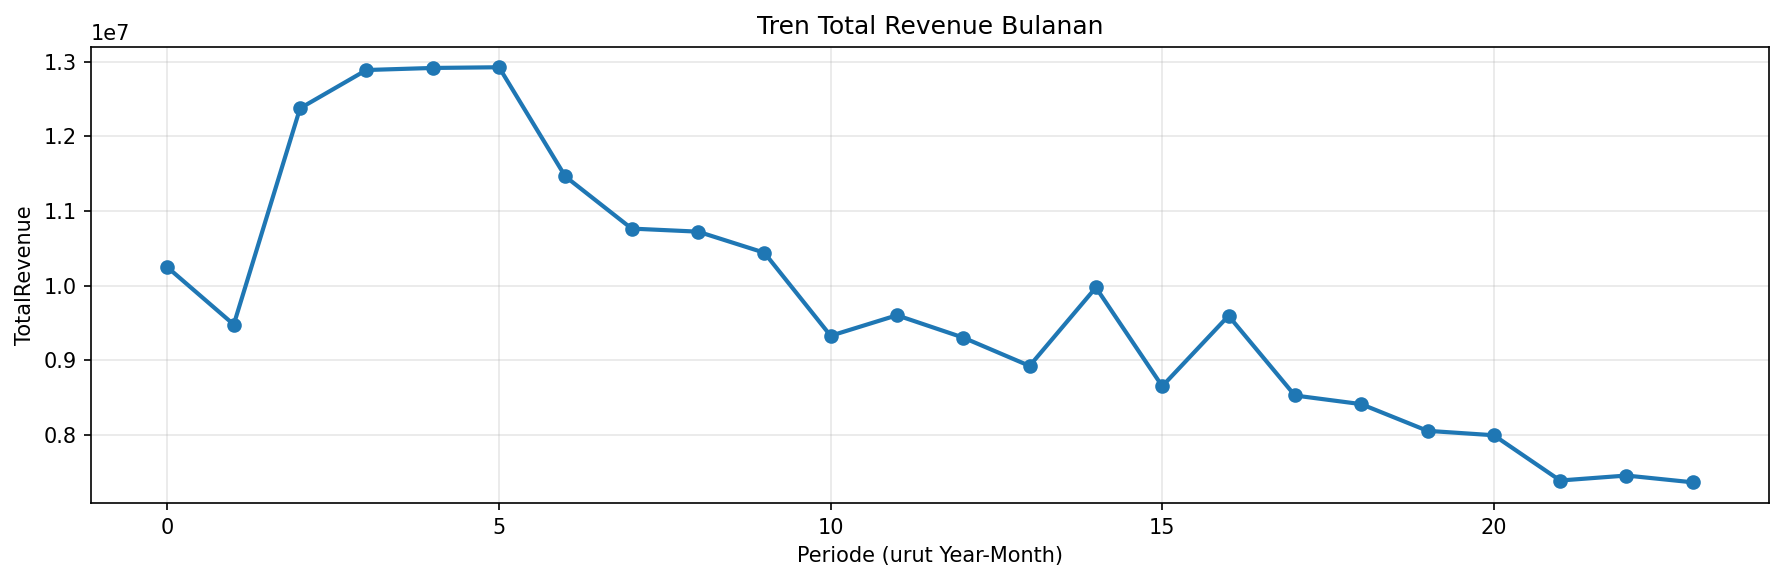
\includegraphics[width=0.92\textwidth]{tugas-akhir/assets/images/tren_revenue.png}
\caption{Pola tren bulanan \texttt{TotalRevenue}}
\label{fig:monthly_revenue_trend}
\end{figure}

\begin{figure}[H]
\centering
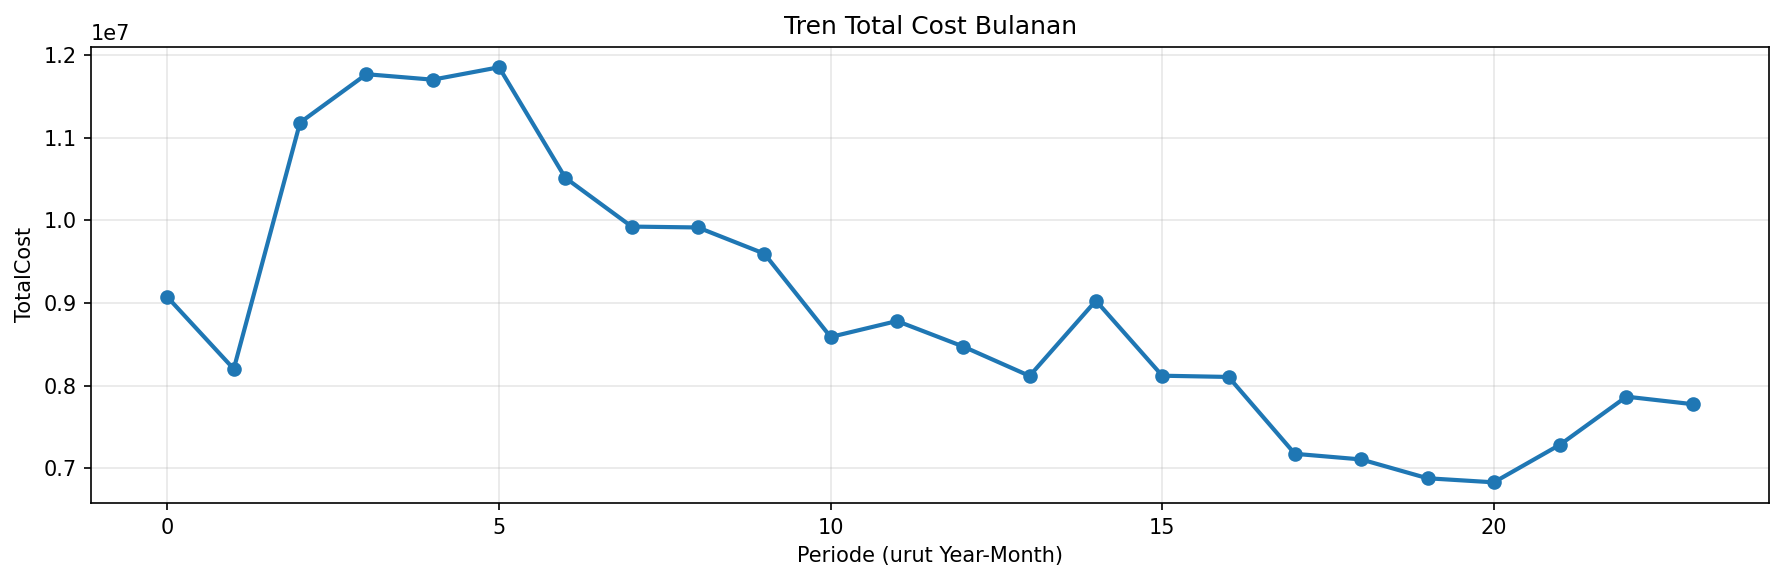
\includegraphics[width=0.92\textwidth]{tugas-akhir/assets/images/tren_cost.png}
\caption{Pola tren bulanan \texttt{TotalCost}}
\label{fig:monthly_cost_trend}
\end{figure}

\begin{figure}[H]
\centering
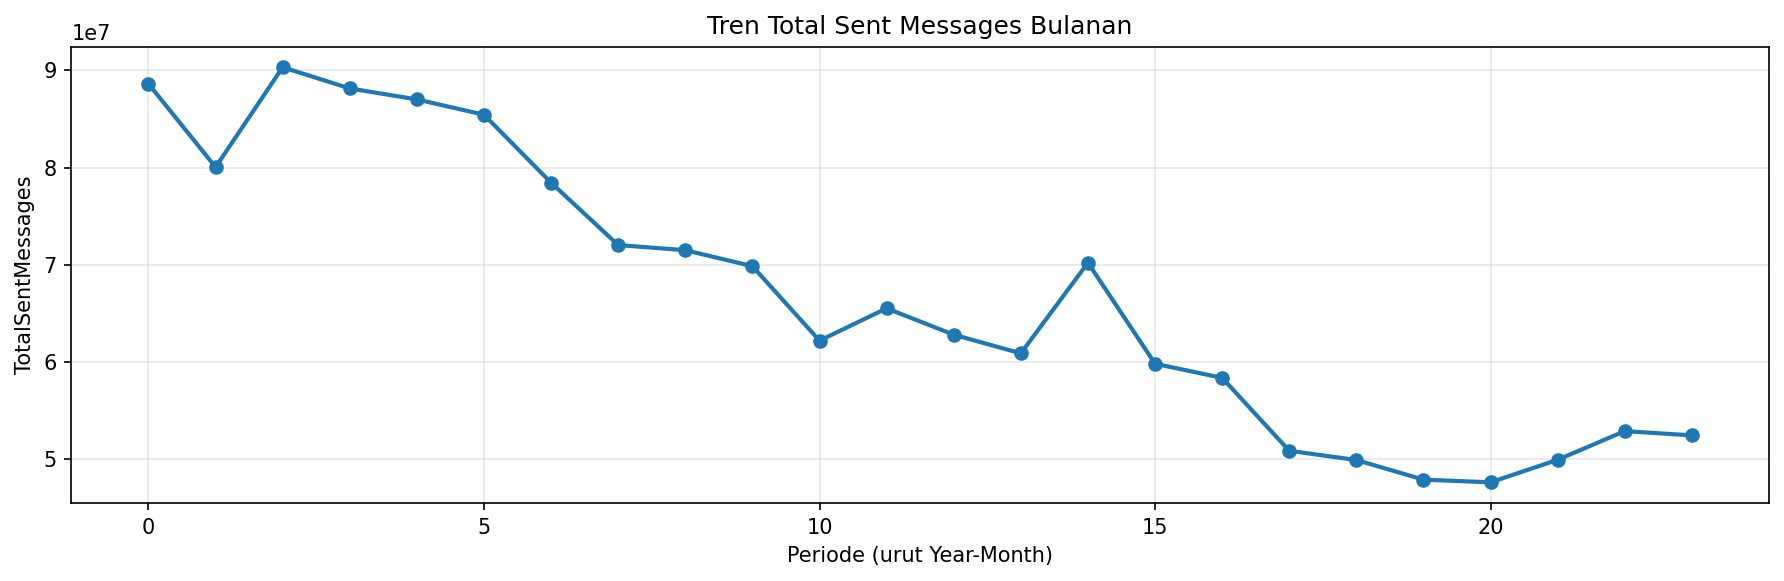
\includegraphics[width=0.92\textwidth]{tugas-akhir/assets/images/tren_sent_messages.png}
\caption{Pola tren bulanan \texttt{TotalSentMessages}}
\label{fig:monthly_sentmessages_trend}
\end{figure}

\begin{figure}[H]
\centering
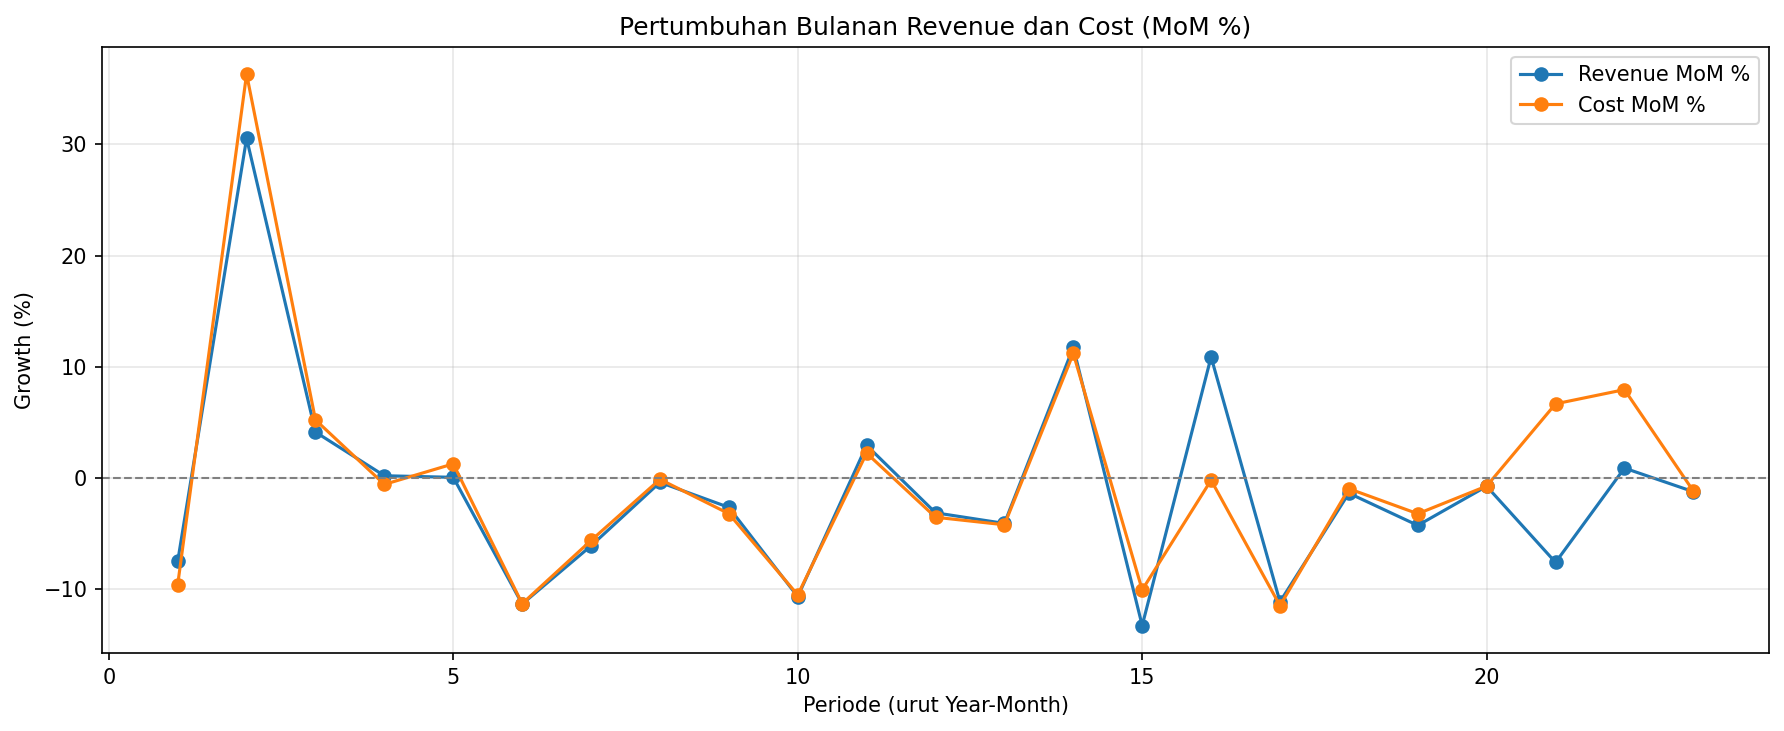
\includegraphics[width=0.92\textwidth]{tugas-akhir/assets/images/tren_mom_growth.png}
\caption{Pola tren bulanan \texttt{TotalSentMessages}}
\label{fig:monthly_monthgrowth_trend}
\end{figure}

Gambar 4.1, 4.2, dan 4.3 menunjukkan pola pertumbuhan bulanan dari kolom target \texttt{TotalRevenue} beserta fitur \texttt{TotalCost} dan \texttt{TotalSentMessages}. Ketiga variabel memperlihatkan tren yang bergerak searah, mengindikasikan adanya korelasi positif yang kuat. Kondisi ini menunjukkan adanya potensi \textit{data leakage} apabila ketiga fitur tersebut digunakan langsung sebagai prediktor untuk memprediksi \texttt{TotalRevenue}. \textit{Data leakage} merupakan kondisi di mana data tertentu secara tidak sengaja memberikan contekan informasi ketika pelatihan model sehingga model terlalu optimis ketika memprediksi data test. Hal ini juga dikuatkan oleh \textit{domain knowledge} yang mana volume pesan yang terkirim dan total biaya secara inheren berkorelasi positif dengan pendapatan yang dihasilkan dari setiap transaksi.
Sedangkan Gambar 4.4 memperkuat temuan tersebut melalui analisis laju pertumbuhan bulanan (\textit{Month-over-Month}, MoM) dari \texttt{TotalRevenue} dan \texttt{TotalCost}. Kedua kurva bergerak hampir beriringan sepanjang periode pengamatan, dengan lonjakan dan penurunan yang terjadi secara bersamaan. Pola sinkronisasi ini menunjukkan bahwa perubahan biaya operasional pada suatu bulan cenderung diikuti oleh perubahan pendapatan pada bulan yang sama, sehingga semakin memperkuat hubungan antara kedua variabel. Selain itu, fluktuasi MoM yang cukup tinggi pada beberapa periode mempresentasikan adanya pola musiman yang perlu dipertimbangkan dalam proses rekayasa fitur temporal.

\subsection{Analisis Distribusi Data}
Analisis distribusi dilakukan untuk memahami sebaran nilai pada variabel kategorikal. Pada analisis ini digunakan \textit{bar chart} untuk melihat distribusi data kategori pada atribut seperti \texttt{Country}, \texttt{Client}, \texttt{Network}, dan \texttt{Route}. Distribusi data kategori dapat dilihat pada persamaan 4.6.
\begin{equation}
\texttt{Count}(c_j) = \sum_{i=1}^{n} \mathbb{I}(C_i = c_j)
\end{equation}

dengan $c_j$ adalah kategori ke-$j$ pada variabel kategorikal $C$. Hasil analisis distribusi menjadi dasar untuk menentukan langkah yang tepat dalam pra-pemrosesan data nantinya.

\begin{figure}[H]
\centering
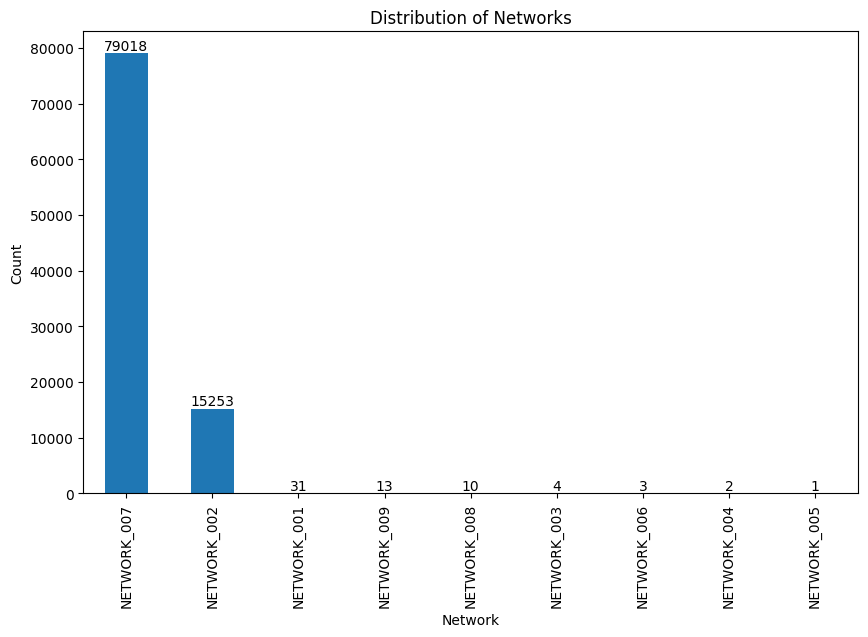
\includegraphics[width=0.7\textwidth]{tugas-akhir/assets/images/distribution-networks.png}
\caption{Distribusi frekuensi transaksi berdasarkan jenis jaringan (\textit{Network})}
\label{fig:distribution_network}
\end{figure}

Gambar 4.5 menunjukkan bahwa \texttt{network-007} memiliki frekuensi transaksi yang jauh lebih tinggi dibandingkan jaringan lainnya, mempresentasikan ketimpangan distribusi yang signifikan. \textit{Insight} yang diperoleh adalah \texttt{network-007} merupakan jaringan yang paling dominan dalam transaksi. Maka dari itu, dapat dianalisis  \texttt{network-007}  merupakan pelanggan utama pada layanan transaksi SMS internasional pada perusahaan X. 

\subsection{Analisis Korelasi Antar Fitur}
Hubungan antar fitur numerik dianalisis menggunakan koefisien korelasi \textit{Pearson}, kemudian divisualisasikan dengan \textit{heatmap}. Nilai korelasi digunakan untuk menilai kekuatan hubungan linear antarvariabel terhadap target \texttt{TotalRevenue}. Koefisien \textit{Pearson} antara dua variabel $X$ dan $Y$ dapat ditulis pada persamaan 4.7.

\begin{equation}
\rho_{X,Y} = \frac{\operatorname{Cov}(X,Y)}{\sigma_X \sigma_Y}
\end{equation}

Dengan nilai $\rho_{X,Y}$ mendekati 1 menunjukkan hubungan positif kuat, mendekati -1 menunjukkan hubungan negatif kuat, dan mendekati 0 menunjukkan hubungan linear lemah.

\begin{figure}[H]
\centering
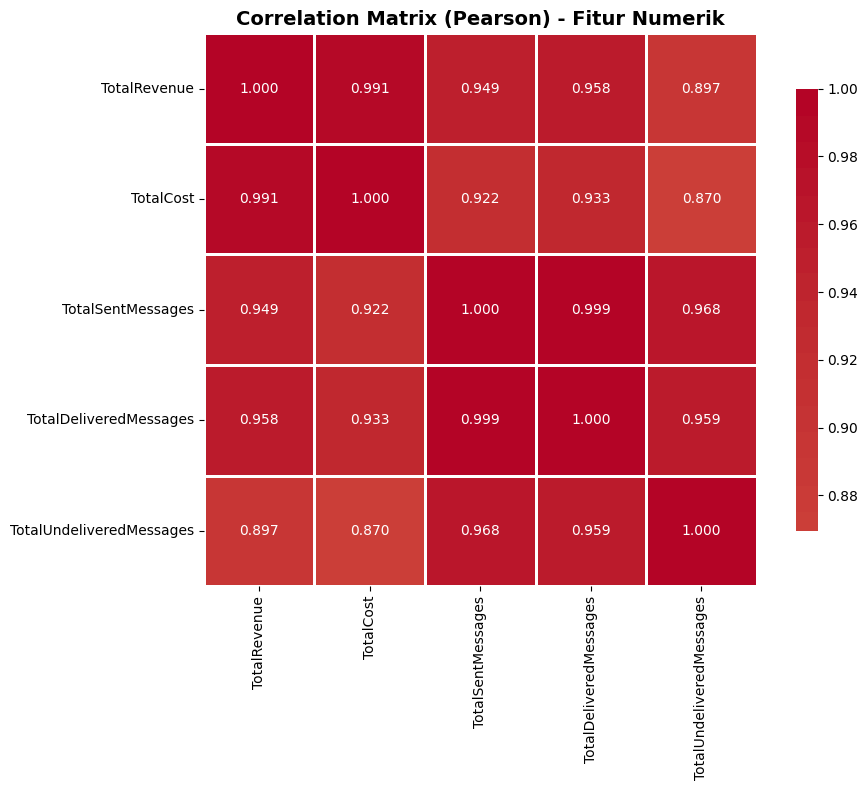
\includegraphics[width=0.7\textwidth]{tugas-akhir/assets/images/analisis-korelasi-antar-fitur.png}
\caption{Nilai Korelasi (hubungan) di tiap fitur numerik}
\label{fig:alur_prapra-pemrosesan}
\end{figure}

Pada gambar 4.6 menunjukkan bahwa korelasi fitur dari keempat fitur numerik yaitu \texttt{TotalCost,TotalSentMessages,TotalDeliveredMessages,TotalUndeliveredMessages}, dengan kolom target sangat tinggi sehingga hal ini menunjukkan data \textit{leakage} jika dipakai untuk proses  \textit{modelling}. Maka dari itu, keempat fitur numerik tersebut tidak digunakan langsung untuk proses \textit{modelling} nantinya.

\subsection{Implikasi EDA terhadap Feature Engineering}
Temuan EDA digunakan sebagai landasan penyusunan fitur model. Pola temporal mendorong pembentukan fitur lag (misalnya \texttt{Prev\_Month\_Volume} dan \texttt{Prev\_Month\_Revenue}), pola distribusi mendukung keputusan pembersihan data dan \textit{encoding kategorikal}, sedangkan pola korelasi membantu memilih fitur yang informatif sekaligus menghindari fitur yang berpotensi memicu \textit{data leakage}. Dengan demikian, EDA tidak hanya berfungsi sebagai tahap deskriptif, tetapi juga sebagai tahapan analitis untuk memastikan fitur yang dibangun relevan dengan data aktual.

% \subsection{Ringkasan Tahapan EDA}
% \begin{table}[htbp]
% \centering
% \caption{Ringkasan Tahapan Exploratory Data Analysis}
% \label{tab:ringkasan_eda}
% \footnotesize
% \begin{tabularx}{\textwidth}{l X X}
% \toprule
% Tahap EDA & Tujuan & Output Analisis \\
% \midrule
% Analisis pola temporal & Mengamati dinamika data lintas waktu & Tren bulanan, lonjakan/penurunan, dan MoM growth \\
% Analisis distribusi data & Memahami sebaran kategori dan numerik & Dominasi kategori, indikasi skewness/outlier \\
% Analisis korelasi antar fitur & Menilai keterkaitan linear antarmetrik & Matriks korelasi, fitur yang paling relevan ke target \\
% % Implikasi ke feature engineering & Menurunkan keputusan fitur berbasis data & Fitur lag, rasio, dan seleksi fitur terarah \\
% \bottomrule
% \end{tabularx}
% \end{table}

% Berdasarkan hasil EDA, data menunjukkan pola yang cukup informatif untuk pemodelan prediktif, sekaligus memberikan dasar yang kuat dalam perancangan fitur dan validasi hipotesis bisnis pada domain trafik SMS International.


\section{Pra-pemrosesan Data}
Tahap pra-pemrosesan data dilakukan untuk memproses data kembali setelah dilakukan proses analisis pola data berdasarkan proses sebelumnya. Proses ini bertujuan agar data yang dimasukkan ke pelatihan model sudah sesuai dan dapat memudahkan model untuk memprediksi kolom target yaitu  \texttt{TotalRevenue}. Proses pra-pemrosesan data terdiri dari penggabungan data berdasarkan bulan dan \textit{feature engineering}.

\subsection{Penggabungan Data Berdasarkan Bulan}
Pada tahap ini dilakukan penggabungan data transaksi ke dalam skala bulanan berdasarkan \texttt{Series\_ID} yang merepresentasikan kombinasi unik \texttt{Client}, \texttt{Route}, \texttt{SupplierConnection}, dan \texttt{Network}. Penggabungan ini diperlukan karena data asli memiliki banyak baris per bulan yang dibedakan oleh \texttt{OAProfiledCategory} sehingga model \textit{tree-based} akan kesulitan mempelajari pola jika harus memprediksi pada tingkat detail tersebut. Dengan diagregasi per bulan, setiap \texttt{Series\_ID} menghasilkan satu observasi per periode bulanan yang bermakna secara bisnis.
Pada proses penggabungan, \texttt{TotalRevenue} dijumlahkan (\textit{sum}) sebagai kolom target prediksi. Kolom \texttt{Client}, \texttt{Route}, \texttt{SupplierConnection}, dan \texttt{Network} digabungkan berdasarkan nilainya identik untuk seluruh baris dalam satu grup sehingga digunakan sebagai kunci grup (\textit{grouping key}) dalam proses \texttt{groupby}. Kolom \texttt{Country} dikeluarkan dari kunci grup karena satu \texttt{Series\_ID} dapat mencakup beberapa \texttt{Country}. Apabila menyertakannya akan memecah agregasi secara tidak diinginkan. Fitur numerik volume yaitu \texttt{TotalCost}, \texttt{TotalProfit}, \texttt{TotalSentMessages}, \texttt{TotalDeliveredMessages}, dan \texttt{TotalUndeliveredMessages} diagregasi dengan \textit{sum} karena secara semantik merupakan akumulasi bulanan yang perlu dijumlahkan. Fitur penanda anomali \texttt{is\_anomaly\_rev\_only} dan \texttt{is\_anomaly\_cost\_only} juga diagregasi dengan \textit{sum} karena jika menggunakan \textit{mode} atau \textit{first}, informasi frekuensi hilang. Sebagai contoh, dua transaksi bonus dalam satu bulan akan terlihat identik dengan satu transaksi bonus. Dengan \textit{sum}, fitur tersebut menjadi dapat menangkap frekuensi kemunculan anomali sehingga lebih informatif bagi model untuk mengenali pola pendapatan yang tidak biasa.
Fitur \texttt{OAProfiledCategory} diagregasi dengan \textit{nunique} menjadi \texttt{unique\_OA\_count} yang menghitung jumlah kategori \textit{OA Profiled} unik dalam satu bulan. Fitur ini merepresentasikan keragaman sub-segmen dalam suatu \texttt{Series\_ID}. Statistik distribusi pendapatan antar kategori OA juga dihitung melalui pre-agregasi, yaitu \texttt{max\_OA\_revenue} dan \texttt{min\_OA\_revenue} masing-masing merupakan pendapatan tertinggi dan terendah dari semua sub-transaksi OA dalam satu grup, memberikan gambaran sebaran data pendapatan per kategori.
Selain itu, dilakukan pembentukan panel lengkap (\textit{complete panel}) di mana setiap \texttt{Series\_ID} memiliki baris untuk semua bulan dalam dataset melalui \textit{cross join} antara daftar \texttt{Series\_ID} unik dan semua kombinasi \textit{Year}--\textit{Month}. Operasi ini menghasilkan semua pasangan \texttt{Series\_ID}--\texttt{Month} yang mungkin, sehingga setiap \texttt{Series\_ID} terwakili di setiap periode meskipun tidak memiliki transaksi pada bulan tersebut. Bulan tanpa transaksi diisi dengan nilai nol pada seluruh kolom numerik. Langkah ini diperlukan karena data asli hanya berisi bulan yang memiliki transaksi, sehingga fitur \textit{lag} akan berisi nilai yang kurang tepat jika bulan kosong tidak direpresentasikan. Berikut merupakan hasil dari penggabungan data transaksi berdasarkan bulan yang dapat dilihat pada Tabel~\ref{tab:monthly_agg}.
\begin{table}[H]
\centering
\caption{Preview Data Agregasi Bulanan}
\label{tab:monthly_agg}
\resizebox{\textwidth}{!}{%
\begin{tabular}{ccrrrrrr}
\toprule
Series\_ID & Year & Month & TotalRevenue & $\cdots$ & unique\_OA\_count & max\_OA\_rev \\
\midrule
CLIENT\_017\_ROUTE\_020\_.. & 2023 & 1 & 610446 & $\cdots$ & 3 & 280000 \\
CLIENT\_017\_ROUTE\_020\_.. & 2023 & 2 & 3153037 & $\cdots$ & 5 & 1500000 \\
CLIENT\_017\_ROUTE\_020\_.. & 2023 & 3 & 2861227 & $\cdots$ & 4 & 1200000 \\
CLIENT\_017\_ROUTE\_020\_.. & 2023 & 4 & 2755164 & $\cdots$ & 2 & 1400000 \\
CLIENT\_017\_ROUTE\_020\_.. & 2023 & 5 & 2716086 & $\cdots$ & 3 & 1350000 \\
\midrule
$\vdots$ & $\vdots$ & $\vdots$ & $\vdots$ & $\cdots$ & $\vdots$ & $\vdots$ \\
\bottomrule
\end{tabular}%
}
\end{table}

\subsection{Rekayasa Fitur (Feature Engineering)}

Pembuatan fitur pada penelitian ini dilakukan dalam tiga tahap yaitu sebelum agregasi bulanan, saat agregasi, dan setelah agregasi. Pada tahap sebelum agregasi, dibangun beberapa fitur pada data transaksi asli yang diperlukan untuk proses penggabungan dan pelabelan anomali.
Pertama, fitur \texttt{Series\_ID} dibentuk dari kombinasi \texttt{Client}, \texttt{Route}, \texttt{SupplierConnection}, dan \texttt{Network} untuk mengelompokkan data (\textit{grouping}) berdasarkan pola waktu masing-masing grup.
\begin{equation}
\texttt{Series\_ID} = \texttt{Client} \oplus \texttt{Route} \oplus \texttt{SupplierConnection} \oplus \texttt{Network}
\end{equation}
\noindent Kolom \texttt{Supplier} tidak disertakan karena hanya memiliki satu jenis data. Kolom \texttt{Country} juga tidak disertakan karena hanya empat baris dari 128 baris yang memiliki \texttt{Country} berbeda (East Timor) dari mayoritas Indonesia pada \texttt{Series\_ID} yang sama, sehingga menyertakannya akan memecah agregasi dan menghasilkan nilai duplikat.
Kedua, fitur penanda anomali dibuat untuk mengidentifikasi transaksi yang memiliki pola yang aneh dan tidak biasa. Pola \textit{bonus} ditandai dengan \texttt{is\_anomaly\_rev\_only} ketika $\texttt{TotalRevenue} \neq 0$, $\texttt{TotalCost} = 0$, dan $\texttt{TotalProfit} = 0$. Pola \textit{testing} ditandai dengan \texttt{is\_anomaly\_cost\_only} ketika $\texttt{TotalRevenue} = 0$, $\texttt{TotalCost} \neq 0$, dan $\texttt{TotalProfit} \neq 0$. Kedua fitur ini bersifat biner ($0$ atau $1$) dan nantinya diagregasi dengan \textit{sum} pada proses penggabungan bulanan.

Setelah penggabungan data berdasarkan bulan, saat aggregasi dibuat fitur-fitur turunan (\textit{derived}) yang tidak dapat dihitung sebelum agregasi karena memerlukan nilai yang telah dijumlahkan. Pertama, fitur rasio biaya per pesan (\texttt{rateCost}) dihitung sebagai berikut.
\begin{equation}
\texttt{rateCost} = 
\begin{cases}
\dfrac{\sum\texttt{TotalCost}}{\sum\texttt{TotalDeliveredMessages}} & \text{jika } \sum\texttt{TotalDeliveredMessages} > 0 \\[8pt]
0 & \text{jika } \sum\texttt{TotalDeliveredMessages} = 0
\end{cases}
\end{equation}
\noindent Perhitungan \texttt{rateCost} dari hasil penjumlahan (\textit{SUM-derived}) lebih akurat dibanding \textit{mean} dari rasio per baris karena memberikan bobot lebih pada baris dengan volume pesan lebih tinggi (\textit{weighted average}).
Kedua, fitur \textit{profit margin} mengukur rasio keuntungan terhadap pendapatan.
\begin{equation}
\texttt{profit\_margin} = 
\begin{cases}
\dfrac{\sum\texttt{TotalProfit}}{\sum\texttt{TotalRevenue}} & \text{jika } \sum\texttt{TotalRevenue} > 0 \\[8pt]
0 & \text{jika } \sum\texttt{TotalRevenue} = 0
\end{cases}
\end{equation}
Ketiga, fitur \textit{delivery rate} menangkap rasio keberhasilan pengiriman pesan, yang menunjukkan performa perusahaan dalam mengelola \textit{traffic} SMS internasional.
\begin{equation}
\texttt{delivery\_rate} = 
\begin{cases}
\dfrac{\sum\texttt{TotalDeliveredMessages}}{\sum\texttt{TotalSentMessages}} & \text{jika } \sum\texttt{TotalSentMessages} > 0 \\[8pt]
0 & \text{jika } \sum\texttt{TotalSentMessages} = 0
\end{cases}
\end{equation}
Keempat, fitur \texttt{anomaly\_count} menghitung total frekuensi kemunculan anomali dalam satu bulan.
\begin{equation}
\texttt{anomaly\_count} = \texttt{is\_anomaly\_rev\_only} + \texttt{is\_anomaly\_cost\_only}
\end{equation}
\noindent di mana \texttt{is\_anomaly\_rev\_only} dan \texttt{is\_anomaly\_cost\_only} merupakan hasil agregasi \textit{sum} dari fitur biner pada data transaksi asli. Terakhir, fitur \texttt{is\_active} ditambahkan sebagai penanda biner yaitu bernilai $1$ jika $\texttt{TotalRevenue} > 0$ dan $0$ jika tidak, sehingga model dapat mempelajari pola \textit{idle}.


Setelah aggregasi, dibangun fitur temporal berbasis \textit{lag} dan \textit{rolling window} pada data bulanan yang telah diurutkan per \texttt{Series\_ID}. Pertama, fitur \textit{lag} menangkap nilai \texttt{TotalRevenue} dan \texttt{is\_active} pada bulan sebelumnya.
\begin{equation}
\texttt{rev\_lag}_{k} = \texttt{TotalRevenue}_{t-k}, \quad k \in \{1, 2, 3\}
\end{equation}
\begin{equation}
\texttt{active\_lag}_{k} = \texttt{is\_active}_{t-k}, \quad k \in \{1, 2, 3\}
\end{equation}
Kedua, fitur \textit{rolling} menangkap tren dan volatilitas pendapatan menggunakan rata-rata bergerak (\textit{rolling mean}) dan simpangan baku bergerak (\textit{rolling standard deviation}) dengan \textit{shift} satu bulan untuk mencegah kebocoran data (\textit{data leakage}).
\begin{equation}
\texttt{rolling\_mean}_{w} = \frac{1}{w}\sum_{i=1}^{w}\texttt{TotalRevenue}_{t-i}, \quad w \in \{3, 6\}
\end{equation}
\begin{equation}
\texttt{rolling\_std}_{w} = \sqrt{\frac{1}{w}\sum_{i=1}^{w}\left(\texttt{TotalRevenue}_{t-i} - \texttt{rolling\_mean}_{w}\right)^{2}}, \quad w \in \{3, 6\}
\end{equation}
Proporsi bulan aktif dalam \textit{window} $w$ dihitung sebagai berikut.
\begin{equation}
\texttt{pct\_active}_{w} = \frac{1}{w}\sum_{i=1}^{w}\texttt{is\_active}_{t-i}, \quad w \in \{3, 6\}
\end{equation}
Ketiga, fitur \texttt{active\_streak} menghitung jumlah bulan berturut-turut \textit{active} hingga bulan sebelumnya, sedangkan \texttt{months\_since\_active} menghitung jumlah bulan sejak terakhir \textit{active}. Terakhir, variabel \textit{month} dienkode secara siklikal untuk menangkap pola musiman.
\begin{equation}
\texttt{month\_sin} = \sin\left(\frac{2\pi \cdot \texttt{Month}}{12}\right), \quad \texttt{month\_cos} = \cos\left(\frac{2\pi \cdot \texttt{Month}}{12}\right)
\end{equation}

% \subsection{Analisis Domain Knowledge}
% Kemudian dibentuk sebuah fitur untuk menangani kondisi anomali pada pola data dengan analisis \textit{domain knowledge}. Contoh kondisi anomali yang diperiksa meliputi ketidakkonsistenan volume pesan dan ketidaksesuaian antara trafik dan nilai finansial. Secara konseptual, indikator anomali dapat dinyatakan sebagai berikut.

% \begin{equation}
% Delete_i =
% \begin{cases}
% \text{True}, & \text{jika } R_i = 0 \land C_i = 0 \land P_i = 0 \\
% \text{False}, & \text{lainnya}
% \end{cases}
% \end{equation}

% \begin{equation}
% \text{is\_anomaly\_cost\_only}_i =
% \begin{cases}
% 1, & \text{jika } R_i = 0 \land (C_i \neq 0 \lor P_i \neq 0) \\
% 0, & \text{lainnya}
% \end{cases}
% \end{equation}

% \begin{equation}
% \text{is\_anomaly\_rev\_only}_i =
% \begin{cases}
% 1, & \text{jika } R_i \neq 0 \land C_i = 0 \land P_i = 0 \\
% 0, & \text{lainnya}
% \end{cases}
% \end{equation}

% Dengan analisis \textit{domain knowledge} didapatkan alasan pemberian nilai tersebut. Jika \texttt{TotalRevenue}, \texttt{TotalCost}, \texttt{TotalProfit} bernilai 0 maka transaksi tersebut merupakan transaksi gagal sehingga nilai yang berpola tersebut bisa dihapus. Kemudian jika \texttt{TotalRevenue} bernilai tidak nol tetapi \texttt{TotalCost} dan \texttt{TotalProfit} bernilai nol, transaksi tersebut dianggap sebagai bonus sehingga nilai tersebut dipertahankan. Untuk menandai transaksi tersebut, ditambahkan fitur baru \texttt{is\_anomaly\_rev\_only} dengan bernilai 1 jika terdapat pola tersebut dan 0 jika tidak. Sedangkan jika \texttt{TotalRevenue} bernilai nol tetapi \texttt{TotalCost} dan \texttt{TotalProfit} memiliki nilai yang berkebalikan, transaksi tersebut dianggap transaksi yang digunakan untuk \textit{testing} (percobaan). Perusahaan telekomunikasi dalam penelitian ini, ketika menyediakan layanan ke beberapa \textit{client}, sudah terbiasa untuk melakukan proses \textit{traffic} SMS secara \textit{testing} . Tujuannya proses \textit{traffic} utama bisa berjalan lebih lancar untuk perusahaan tertentu.  Sama seperti fitur sebelumnya, untuk menandai transaksi tersebut ditambahkan fitur baru \texttt{is\_anomaly\_cost\_only} dengan bernilai 1 jika terdapat pola tersebut dan 0 jika tidak.

\begin{table}[H]
  \centering
  \caption{Preview Data Setelah Proses \textit{Feature Engineering} (5 Baris Pertama)}
  \label{tab:df_final_preview}
  \resizebox{\textwidth}{!}{%
  \begin{tabular}{c|c|c|c|c|c|c|c}
    \hline
    Client\_enc & $\cdots$ & rateCost & is\_anomaly\_rev\_only & is\_anomaly\_cost\_only & Series\_ID & Month \& Year & TotalRevenue \\
    \hline
    28 & $\cdots$ & 0.137437 & 0 & 0 & CLIENT\_030\_ROUTE\_037\_SC\_001 & 1, 2023 & 1{,}098{,}604 \\
    12 & $\cdots$ & 0.104801 & 0 & 0 & CLIENT\_013\_ROUTE\_016\_SC\_004 & 1, 2023 & 810{,}829 \\
    12 & $\cdots$ & 0.104805 & 0 & 0 & CLIENT\_013\_ROUTE\_016\_SC\_004 & 1, 2023 & 810{,}779 \\
    12 & $\cdots$ & 0.103173 & 0 & 0 & CLIENT\_013\_ROUTE\_016\_SC\_004 & 1, 2023 & 753{,}265 \\
    12 & $\cdots$ & 0.103182 & 0 & 0 & CLIENT\_013\_ROUTE\_016\_SC\_004 & 1, 2023 & 752{,}645 \\
    \hline
  \end{tabular}%
  }
\end{table}

% =============================================================
% BAB 4.5 - PELATIHAN MODEL
% =============================================================

\section{Pelatihan Model}
\label{subsec:pelatihan_model}

Tahap pelatihan model pada penelitian ini menggunakan pendekatan \textit{two-stage model}. Tahap pertama (\textit{Stage 1}) adalah klasifikasi biner untuk memprediksi apakah suatu \texttt{Series\_ID} akan aktif pada bulan berikutnya dan tahap kedua (\textit{Stage 2}) adalah regresi untuk memprediksi nilai \texttt{TotalRevenue} hanya pada \texttt{Series\_ID} yang diprediksi aktif (pendapatan tidak nol). Pendekatan ini dipilih karena sebagian besar \texttt{Series\_ID} mengalami periode \textit{idle} (tidak aktif), sehingga model regresi yang memprediksi pendapatan secara langsung tanpa tahap penyaringan akan mengalami bias yang signifikan. Prediksi akhir merupakan hasil perkalian keluaran klasifikasi dengan keluaran regresi. Apabila $P = 0$ maka prediksi akhir bernilai nol, sedangkan apabila $P = 1$ maka prediksi akhir sama dengan keluaran regresi. Skema pelatihan model secara keseluruhan ditunjukkan pada Gambar 4.7.

\begin{figure}[htbp]
\centering
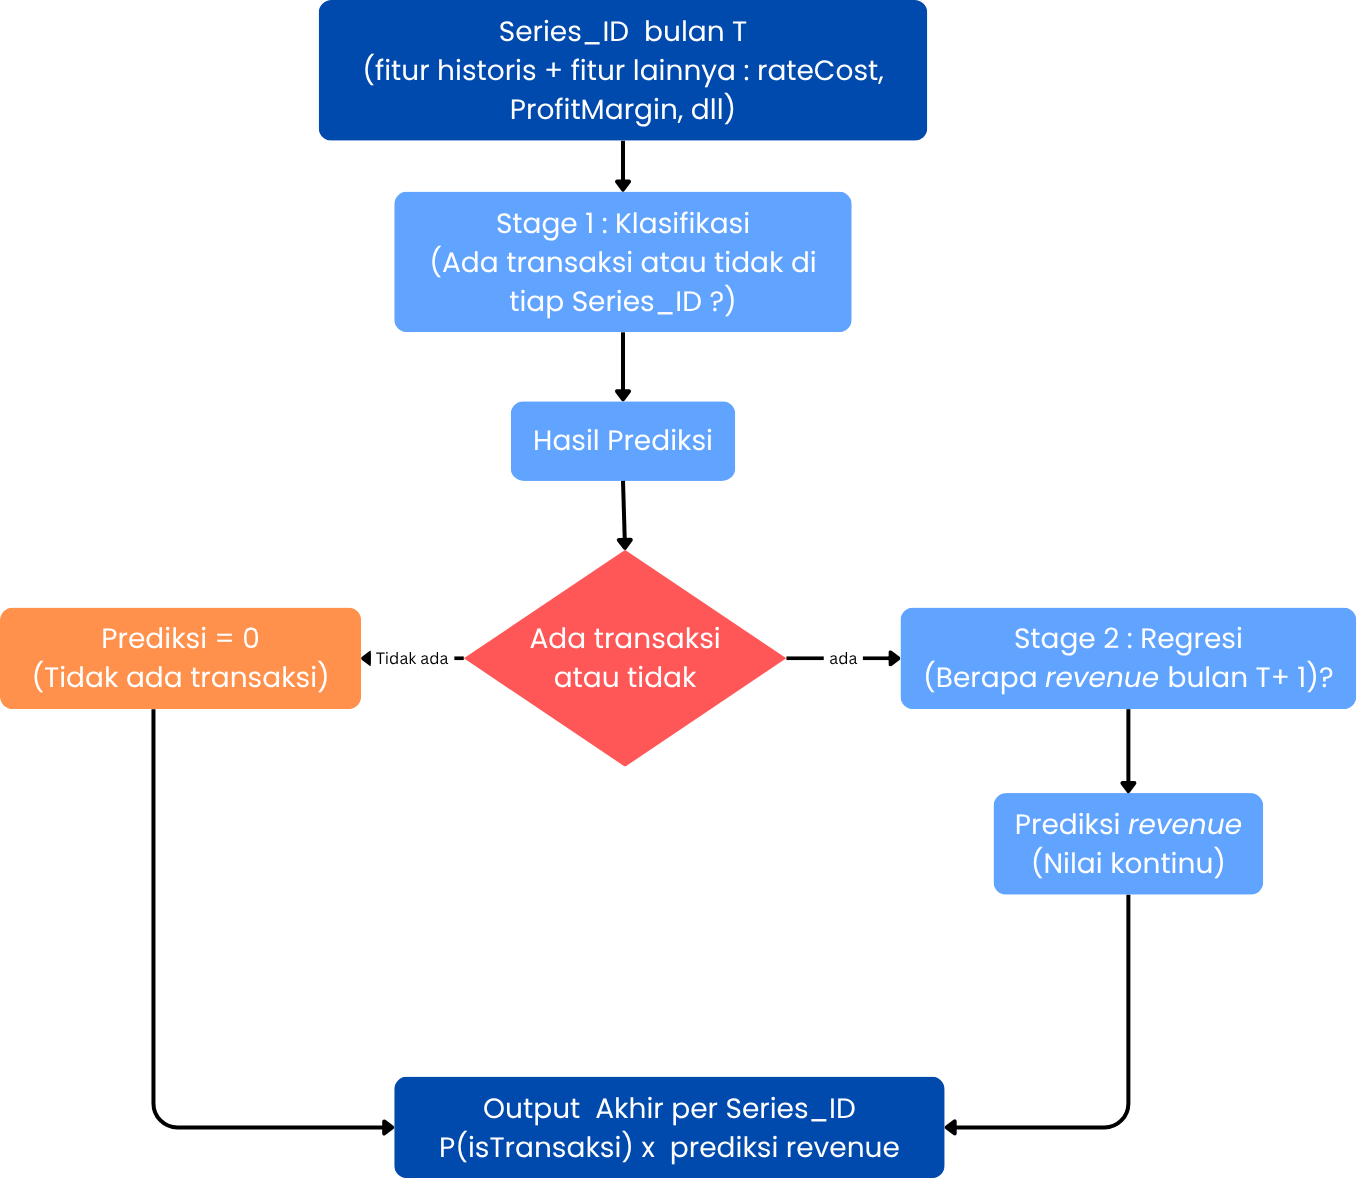
\includegraphics[width=0.92\textwidth]{tugas-akhir/assets/images/skemapelatihanmodel.png}
\caption{Skema pendekatan \textit{two-stage model} untuk prediksi \textit{TotalRevenue}}
\label{fig:skema_pelatihan_model}
\end{figure}

Data dibagi secara kronologis menggunakan kolom \textit{period} ($\texttt{Year} \times 12 + \texttt{Month}$). Titik pemisahan (\textit{cutoff}) ditetapkan pada persentil ke-80 dari kolom \textit{period}, menghasilkan sekitar 80\% data latih dan 20\% data uji dan secara tepatnya ada 1729 data latih dan 364 data uji. Pendekatan ini memastikan bahwa data latih selalu mendahului data uji secara kronologis, sehingga tidak ada informasi dari masa depan yang bocor (\textit{leakage}) ke dalam model. Kedua tahap menggunakan pembagian data yang sama, dengan penyesuaian di tahap kedua hanya memanfaatkan baris dengan \texttt{target\_active} = 1 pada data latih dan baris yang diprediksi aktif pada data uji.

Metrik evaluasi utama yang digunakan konsisten dengan fungsi \textit{fitness} GA, yaitu \textit{Weighted Mean Absolute Percentage Error} (WMAPE). WMAPE dipilih karena mengakomodasi perbedaan skala nilai pendapatan antar \texttt{Series\_ID}, sehingga kesalahan prediksi pada \texttt{Series\_ID} yang memiliki total nilai aktual bernilai besar mendapat bobot proporsional yang lebih tinggi. Selain WMAPE, metrik pendukung yang digunakan meliputi MAE dan $R^2$.

% ---------------------------------------------------------
\subsection{Klasifikasi Transaksi Aktif dan Tidak Aktif}
\label{subsubsec:stage1_klasifikasi}

Pada tahap ini \textit{tree-based models} bertugas mengklasifikasikan apakah suatu \texttt{Series\_ID} akan aktif (\texttt{target\_active} = 1) atau \textit{idle} (\texttt{target\_active} = 0) pada bulan berikutnya. Klasifikasi ini penting karena hanya \texttt{Series\_ID} yang diprediksi aktif yang akan diteruskan ke tahap kedua untuk prediksi pendapatan. \textit{tree-based models} yang digunakan pada tahap ini adalah \textit{XGBoost}. \textit{XGBoost} dipilih karena model ini memiliki parameter \textit{scale\_pos\_weight} yang penting untuk mengatasi ketidakseimbangan kelas antara \texttt{Series\_ID} aktif dan \textit{idle}, memiliki mekanisme \textit{early stopping} yang mencegah \textit{overfitting}, dan sering digunakan untuk memecahkan permasalahan \textit{machine learning} pada data tabular.

Paramater model \textit{XGBoost} yang digunakan pada tahap ini yaitu \texttt{n\_estimators} = 1000, \texttt{learning\_rate} = 0{,}3, \texttt{max\_depth} = 6, \texttt{subsample} = 1{,}0, \texttt{colsample\_bytree} = 1{,}0, \texttt{reg\_lambda} = 1{,}0, \texttt{scale\_pos\_weight} = rasio kelas (\textit{idle}/\textit{active}), \texttt{random\_state} = 42. Parameter \texttt{scale\_pos\_weight} dihitung secara otomatis sebagai rasio jumlah \texttt{Series\_ID} \textit{idle} terhadap \texttt{Series\_ID} aktif pada data latih untuk mengatasi ketidakseimbangan kelas. \textit{Early stopping} dengan \textit{patience} 50 iterasi diterapkan pada data uji untuk menghentikan pelatihan jika tidak ada peningkatan performansi model. 

Fitur yang digunakan pada tahap ini terdiri dari 20 fitur. Fitur ini merupakan hasil dari pra-pemrosesan data dan \textit{feature engineering} dari proses sebelumnya. Fitur ini dapat dikelompokkan sebagai berikut.
\begin{enumerate}
    \item Status historis : \texttt{active\_lag1}, \texttt{active\_lag2}, \texttt{active\_lag3}, \texttt{active\_streak}, \texttt{months\_since\_active}, \texttt{pct\_active\_3m}, \texttt{pct\_active\_6m}
    \item \textit{Revenue} historis : \texttt{rev\_lag1}, \texttt{rev\_lag2}, \texttt{rev\_lag3}, \texttt{rolling\_mean\_3}, \texttt{rolling\_mean\_6} 
    \item Operasional : \texttt{TotalSentMessages}, \texttt{TotalDeliveredMessages}, \texttt{delivery\_rate}, \texttt{unique\_OA\_count}
    \item Anomali : \texttt{anomaly\_count}, \texttt{anomaly\_revenue\_pct}
    \item Siklikalitas : \texttt{month\_sin}, \texttt{month\_cos}.
\end{enumerate}

Metrik evaluasi pada tahap ini menggunakan ROC-AUC dan PR-AUC yang dipilih karena data memiliki ketidakseimbangan kelas antara transaksi aktif (994 data) dan tidak aktif (1.099 data). Hasil evaluasi menunjukkan ROC-AUC sebesar 0,9611 dan PR-AUC sebesar 0,9748, yang menunjukan performa klasifikasi yang sangat baik dalam membedakan transaksi aktif dari yang \textit{idle} meskipun terdapat ketidakseimbangan kelas.

% ---------------------------------------------------------
\subsection{Regresi Pendapatan}
\label{subsubsec:stage2_regresi}

Pada tahap ini \textit{tree-based models} bertugas memprediksi nilai pendapatan (\texttt{target\_revenue}) hanya untuk \texttt{Series\_ID} yang diklasifikasikan aktif atau bernilai bukan nol. \textit{Tree-based models} yang digunakan adalah \textit{Random Forest} dan \textit{XGBoost}. Data train untuk tahap ini disaring sehingga hanya memuat \texttt{Series\_ID} yang aktif pada data latih (\texttt{target\_active} = 1). Sedangkan pada data uji, data yang digunakan berdasarkan prediksi pada tahap pertama, sehingga mensimulasikan proses \textit{inferensi} (pengujian) yang sebenarnya.

Fitur yang digunakan pada tahap kedua identik dengan tahap pertama ditambah dengan \texttt{rateCost}, \texttt{unique\_OA\_count}, \texttt{max\_OA\_revenue} sehingga total ada 23 fitur. Hasil pelatihan model \textit{baseline} pada tahap ini menunjukkan \textit{XGBoost} mencapai WMAPE 27,68\%, $R^2$ 0,920, dan MAE 39.582,76, sedangkan \textit{Random Forest} mencapai WMAPE 24,82\%, $R^2$ 0,932, dan MAE 35.485,88. Dengan demikian, \textit{Random Forest baseline} mengungguli \textit{XGBoost baseline} pada semua metrik evaluasi. Performa kedua model \textit{baseline} ini menjadi acuan pembanding untuk mengevaluasi efektivitas optimasi hiperparameter menggunakan Algoritma Genetika.

% =============================================================
% BAB 4.6 - OPTIMASI HYPERPARAMETER MENGGUNAKAN ALGORITMA GENETIKA
% =============================================================

% \section{Optimasi Hiperparameter dengan Algoritma Genetika}
% \label{subsec:optimasi_hyperparameter}

% Untuk menentukan konfigurasi hiperparameter yang optimal, penelitian ini menerapkan Algoritma Genetika pada dua model \textit{tree-based} yaitu \textit{Random Forest} (berbasis \textit{bagging ensemble}) dan XGBoost (berbasis \textit{boosting ensemble}). Pemilihan kedua model ini memungkinkan perbandingan efektivitas GA pada dua paradigma \textit{ensemble} yang berbeda. Hal serupa dilakukan oleh Mansoori (2023) yang membandingkan performa \textit{tree-based models} dalam konteks prediksi durasi perawatan di rumah sakit.

% GA dijalankan secara independen untuk masing-masing model dengan konfigurasi 20 individu per populasi, 50 generasi, \textit{crossover rate} = 1,0, \textit{mutation rate} = 0,2, dan \textit{keep\_elitism} = 2. Setelah 50 generasi, konfigurasi hiperparameter optimal berhasil ditemukan untuk setiap model dan dibandingkan dengan performa model \textit{baseline}.

% Kedua model dilakukan evaluasi pada data uji di tahap 2 menggunakan empat model yaitu \textit{Random Forest Baseline}, \textit{Random Forest + GA}, \textit{XGBoost Baseline}, dan \textit{XGBoost + GA}. Hasil optimasi menunjukkan peningkatan yang signifikan pada kedua model. Pada \textit{Random Forest}, WMAPE turun dari 24,82\% menjadi 18,80\% (reduksi 6,02 poin persentase), $R^2$ meningkat dari 0,9315 menjadi 0,9717, dan MAE turun dari 35.485,88 menjadi 26.890,63. Pada XGBoost, WMAPE turun dari 27,68\% menjadi 15,46\% (reduksi 12,22 poin persentase), $R^2$ meningkat dari 0,9207 menjadi 0,9907, dan MAE turun dari 39.582,76 menjadi 22.107,41. Model \textit{XGBoost + GA} memberikan performa terbaik secara keseluruhan dengan WMAPE terendah (15,46\%), RMSE terendah (46.823,86), dan $R^2$ tertinggi (0,9907). Besarnya peningkatan pada XGBoost (12,22 poin persentase) yang lebih besar dibandingkan \textit{Random Forest} (6,02 poin persentase) mengindikasikan bahwa konfigurasi \textit{default} XGBoost kurang optimal untuk karakteristik data ini, sehingga XGBoost mengalami pertumbuhan performa yang signifikan dari proses optimasi hiperparameter oleh GA. Tabel \ref{tab:perbandingan_model} menyajikan perbandingan performa keempat model.

% \begin{table}[H]
% \centering
% \caption{Perbandingan Hasil Evaluasi Model Tahap Kedua}
% \label{tab:perbandingan_model}
% \begin{tabular}{llccc}
% \toprule
% \textbf{Model} & \textbf{Konfigurasi} & \textbf{WMAPE (\%)} & \textbf{$R^2$} & \textbf{MAE} \\
% \midrule
% Random Forest  & Baseline  & 24,82 & 0,9315 & 35\,485,88 \\
% Random Forest  & GA-Tuned  & 18,80 & 0,9717 & 26\,890,63 \\
% XGBoost        & Baseline  & 27,68 & 0,9207 & 39\,582,76 \\
% XGBoost        & GA-Tuned  & 15,46 & 0,9907 & 22\,107,41 \\
% \bottomrule
% \end{tabular}
% \end{table}

% Untuk mendapatkan gambaran yang lebih komprehensif mengenai distribusi kesalahan prediksi, analisis visual menggunakan \textit{boxplot} dilakukan sebagaimana ditunjukkan pada Gambar 4.8. Hasil visualisasi mengkonfirmasi bahwa model \textit{XGBoost + GA} memiliki rata-rata \textit{error} yang paling rendah dan distribusi kesalahan yang paling terpusat dibandingkan model lainnya. Untuk melengkapi analisis, indeks statistik deskriptif --- meliputi rata-rata, median, standar deviasi, \textit{interquartile range}, nilai minimum, dan maksimum --- juga dihitung untuk setiap model \cite{https://doi.org/10.1155/2023/9673395}. Gambar 4.9 menunjukkan bahwa \textit{XGBoost + GA} tetap unggul berdasarkan semua indeks statistik. Sebagai perbandingan, \textit{XGBoost baseline} memiliki nilai maksimum kesalahan yang sangat tinggi, menunjukkan ketidakstabilan prediksi yang berhasil diatasi oleh optimasi GA.

% \begin{figure}[H]
% \centering
% 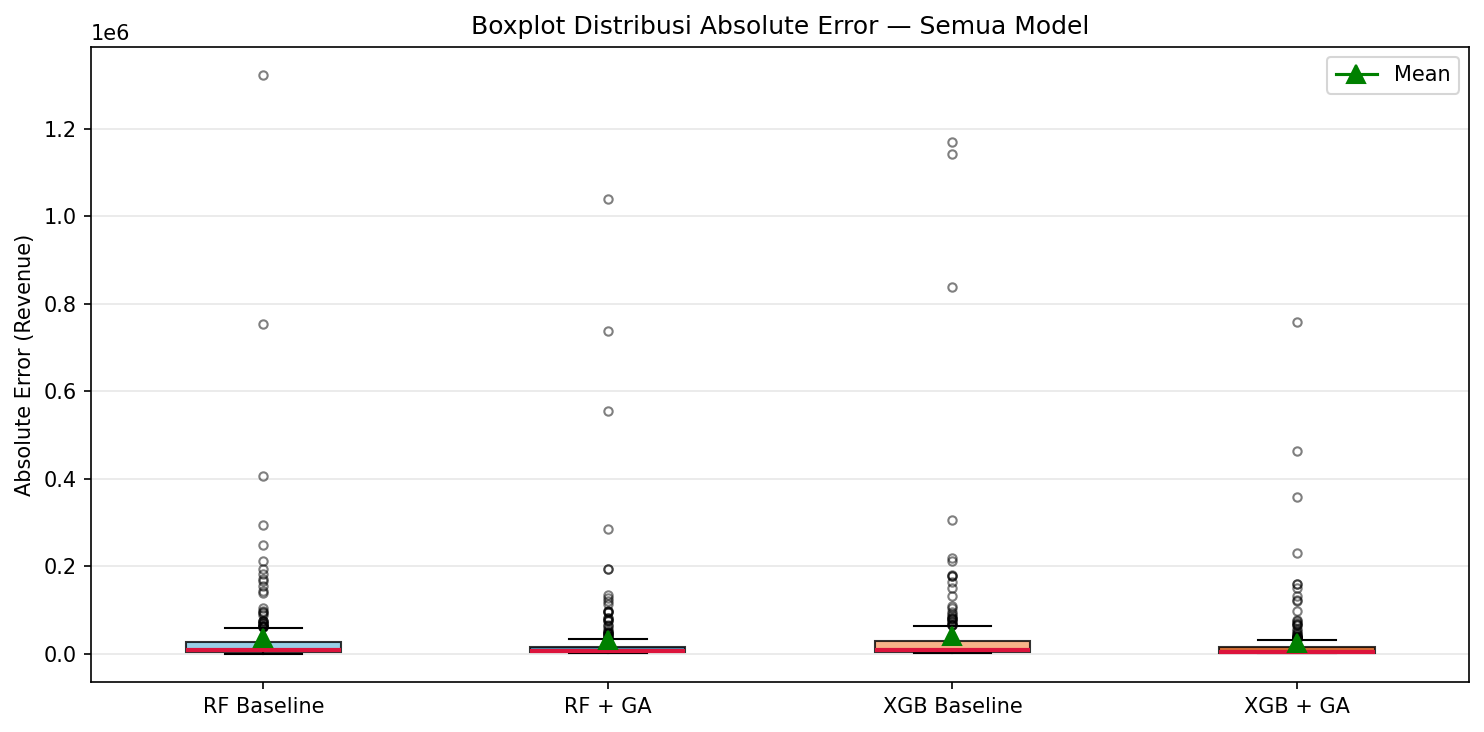
\includegraphics[width=0.7\textwidth]{tugas-akhir/assets/images/boxplot_error_models.png}
% \caption{Perbandingan distribusi kesalahan prediksi (\textit{boxplot error}) keempat model}
% \label{fig:boxplot_error}
% \end{figure}

% \begin{figure}[H]
% \centering
% 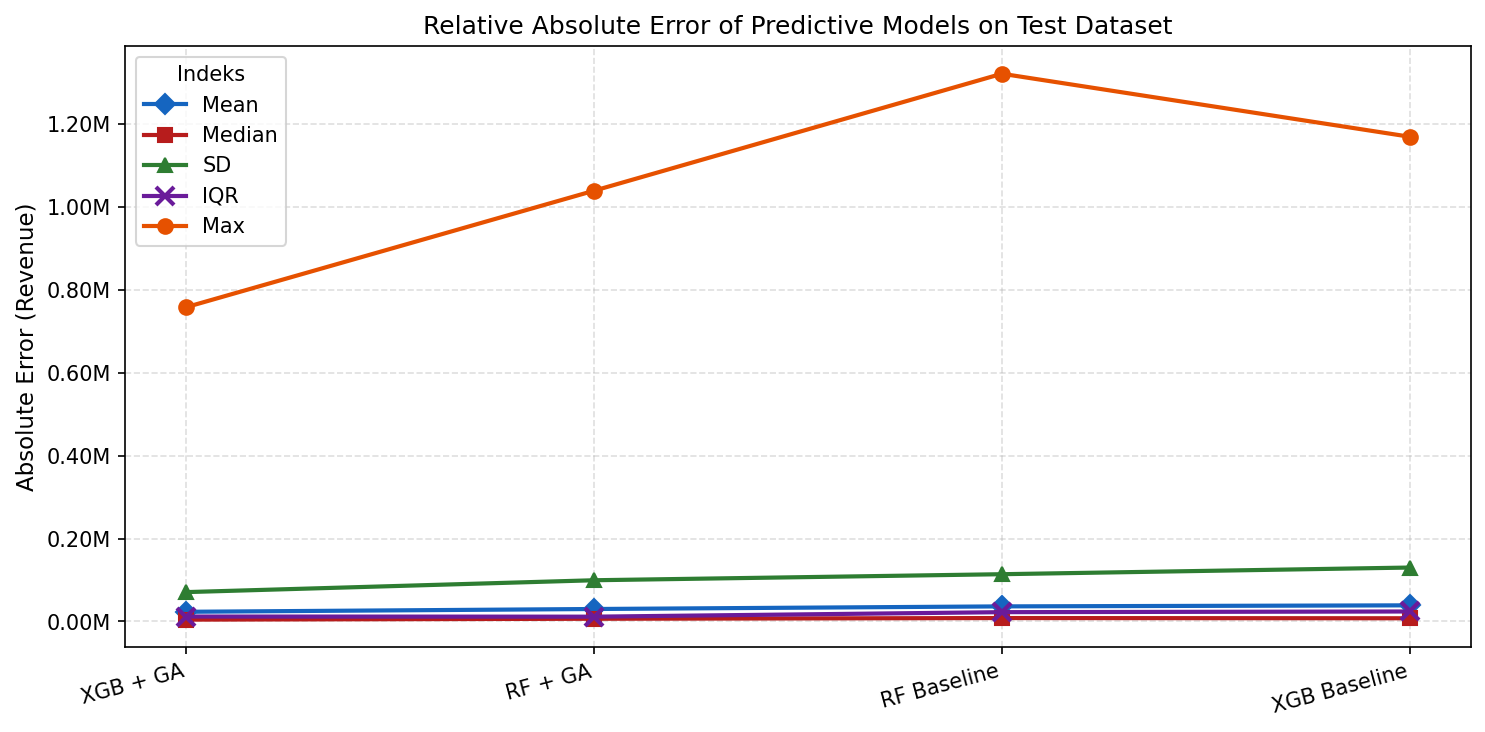
\includegraphics[width=0.7\textwidth]{tugas-akhir/assets/images/relative_absolute_error.png}
% \caption{Indeks statistik deskriptif kesalahan prediksi seluruh model}
% \label{fig:relative_absolute_error}
% \end{figure}

% Selain analisis kesalahan, kurva konvergensi GA ditunjukkan pada Gambar 4.10. Kurva ini memperlihatkan peningkatan nilai fungsi \textit{fitness} yang konsisten di setiap generasi untuk kedua model, mengkonfirmasi bahwa GA berhasil menavigasi ruang pencarian hiperparameter secara efektif. Konfigurasi hiperparameter optimal yang dihasilkan GA untuk masing-masing model ditunjukkan pada Tabel 4.10 dan Tabel 4.11.

% \begin{figure}[H]
% \centering
% 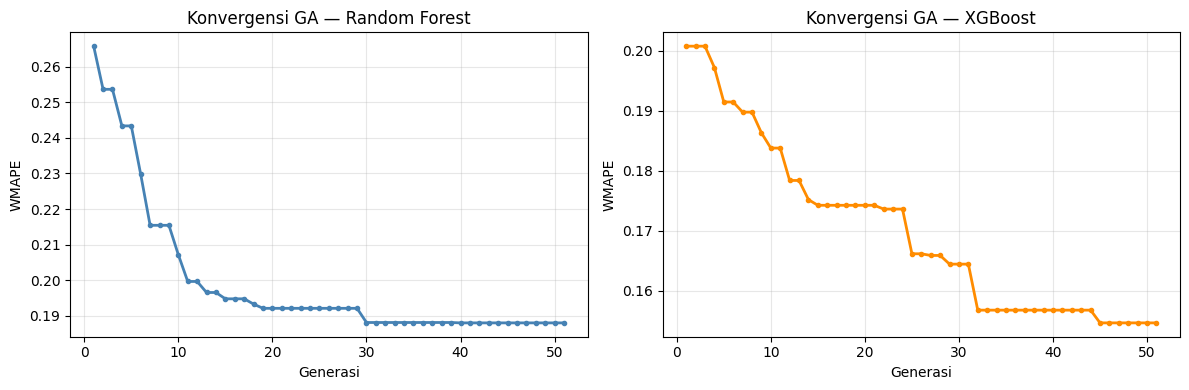
\includegraphics[width=0.92\textwidth]{tugas-akhir/assets/images/output_konvergensi_ga.png}
% \caption{Kurva konvergensi fungsi \textit{fitness} GA untuk \textit{Random Forest} dan \textit{XGBoost}}
% \label{fig:ga_convergence}
% \end{figure}

% \begin{table}[h!]
% \centering
% \caption{Hiperparameter optimal \textit{Random Forest Regressor} hasil GA}
% \label{tab:optimal_hp_rf}
% \begin{tabular}{llc}
% \toprule
% \textbf{Hiperparameter} & \textbf{Ruang Pencarian} & \textbf{Nilai Optimal} \\
% \midrule
% \texttt{n\_estimators}       & [50, 1000]    & 115   \\
% \texttt{max\_depth}          & [1, 7]         & 7     \\
% \texttt{min\_samples\_split} & [2, 20]        & 4     \\
% \texttt{min\_samples\_leaf}  & [1, 50]        & 2     \\
% \texttt{max\_features}       & [1, $N_f$]     & 6     \\
% \texttt{max\_samples}        & [0{,}1, 1{,}0] & 0{,}877 \\
% \bottomrule
% \end{tabular}
% \end{table}

% \begin{table}[h!]
% \centering
% \caption{Hiperparameter optimal \textit{XGBoost Regressor} hasil GA}
% \label{tab:optimal_hp_xgb}
% \begin{tabular}{llc}
% \toprule
% \textbf{Hiperparameter} & \textbf{Ruang Pencarian} & \textbf{Nilai Optimal} \\
% \midrule
% \texttt{learning\_rate}      & [0{,}001, 1{,}0]     & 0{,}224 \\
% \texttt{n\_estimators}       & [50, 1000]           & 462   \\
% \texttt{max\_depth}          & [1, 7]                & 5     \\
% \texttt{subsample}           & [0{,}1, 1{,}0]       & 0{,}756 \\
% \texttt{colsample\_bytree}   & [0{,}1, 1{,}0]       & 0{,}631 \\
% \texttt{reg\_lambda}         & [1, 3]                & 1{,}506 \\
% \bottomrule
% \end{tabular}
% \end{table}

\section{Optimasi \textit{Hyperparameter} dengan Algoritma Genetika}
\label{subsec:optimasi_hyperparameter}

Untuk menentukan konfigurasi hiperparameter yang optimal, penelitian ini menerapkan Algoritma Genetika pada dua model \textit{tree-based} yaitu \textit{Random Forest} (berbasis \textit{bagging ensemble}) dan XGBoost (berbasis \textit{boosting ensemble}). Pemilihan kedua model ini memungkinkan perbandingan efektivitas GA pada dua paradigma \textit{ensemble} yang berbeda. Hal serupa dilakukan oleh Mansoori (2023) yang membandingkan performa kedua model dalam konteks prediksi durasi perawatan di rumah sakit.

GA dijalankan secara independen untuk masing-masing model dengan konfigurasi yang identik yaitu 40 individu per populasi, 100 generasi, \textit{crossover rate} = 1,0, \textit{mutation rate} = 0,2, dan \textit{keep\_elitism} = 2. Setelah 100 generasi, konfigurasi \textit{hyperparameter} optimal berhasil ditemukan untuk setiap model dan dibandingkan dengan performa model \textit{baseline}.

% ---------------------------------------------------------
\subsection{Representasi Kromosom dan Ruang Pencarian}
\label{subsec:kromosom_ga}

Setiap individu dalam populasi GA direpresentasikan sebagai kromosom berupa vektor real $\boldsymbol{\theta} \in \mathbb{R}^6$, di mana masing-masing gen memetakan satu \textit{hyperparameter}. Kedua model dioptimalkan secara terpisah dengan ruang pencarian yang berbeda. Untuk lebih detailnya dapat dilihat pada Tabel~\ref{tab:gene_rf} dan \ref{tab:gene_xgb}.

\begin{table}[h!]
\centering
\caption{Ruang pencarian kromosom \textit{Random Forest Regressor}}
\label{tab:gene_rf}
\begin{tabular}{clccc}
\toprule
\textbf{Gen ke-} & \textbf{\textit{Hyperparameter}} & \textbf{Tipe} & \textbf{Min} & \textbf{Maks} \\
\midrule
0 & \texttt{n\_estimators}       & Integer & 50    & 1.000 \\
1 & \texttt{max\_depth}          & Integer & 1     & 7     \\
2 & \texttt{min\_samples\_split} & Integer & 2     & 20    \\
3 & \texttt{min\_samples\_leaf}  & Integer & 1     & 50    \\
4 & \texttt{max\_features}       & Integer & 1     & $N_f$ \\
5 & \texttt{max\_samples}        & Float   & 0{,}1 & 1{,}0 \\
\bottomrule
\end{tabular}
\end{table}

\begin{table}[h!]
\centering
\caption{Ruang pencarian kromosom \textit{XGBoost Regressor}}
\label{tab:gene_xgb}
\begin{tabular}{clccc}
\toprule
\textbf{Gen ke-} & \textbf{\textit{Hyperparameter}} & \textbf{Tipe} & \textbf{Min} & \textbf{Maks} \\
\midrule
0 & \texttt{learning\_rate}    & Float   & 0{,}001 & 1{,}0 \\
1 & \texttt{n\_estimators}     & Integer & 50      & 1.000 \\
2 & \texttt{max\_depth}        & Integer & 1       & 7     \\
3 & \texttt{subsample}         & Float   & 0{,}1   & 1{,}0 \\
4 & \texttt{colsample\_bytree} & Float   & 0{,}1   & 1{,}0 \\
5 & \texttt{reg\_lambda}       & Float   & 1       & 3     \\
\bottomrule
\end{tabular}
\end{table}

Sebagai ilustrasi proses representasi kromosom, sebuah individu dalam populasi memiliki kromosom \textit{Random Forest} dengan nilai gen kontinu sebagai berikut.

\begin{equation}
\boldsymbol{\theta} = [312{,}4;\ 5{,}2;\ 13{,}7;\ 7{,}8;\ 4{,}3;\ 0{,}62]
\end{equation}

Fungsi \texttt{decode\_rf()} mengonversi nilai gen ke \textit{hyperparameter} melalui pembulatan (\textit{round}) untuk tipe integer dan pemotongan (\textit{clip}) ke batas rentang yang valid.

\begin{align}
\texttt{n\_estimators}       &= \operatorname{clip}\!\left(\operatorname{round}(312{,}4),\ 50,\ 1000\right) = 312 \nonumber \\
\texttt{max\_depth}          &= \operatorname{clip}\!\left(\operatorname{round}(5{,}2),\ 1,\ 7\right)       = 5   \nonumber \\
\texttt{min\_samples\_split} &= \operatorname{clip}\!\left(\operatorname{round}(13{,}7),\ 2,\ 20\right)     = 14  \nonumber \\
\texttt{min\_samples\_leaf}  &= \operatorname{clip}\!\left(\operatorname{round}(7{,}8),\ 1,\ 50\right)      = 8   \nonumber \\
\texttt{max\_features}       &= \operatorname{clip}\!\left(\operatorname{round}(4{,}3),\ 1,\ N_f\right)     = 4   \nonumber \\
\texttt{max\_samples}        &= \operatorname{clip}(0{,}62,\ 0{,}1,\ 1{,}0)                               = 0{,}62
\end{align}

% Kromosom optimal yang ditemukan GA setelah 50 generasi untuk \textit{Random Forest} adalah:
% \begin{equation}
% \boldsymbol{\theta}^{*}_{\text{RF}} = [115;\ 7;\ 4;\ 2;\ 6;\ 0{,}877]
% \end{equation}
% dan untuk \textit{XGBoost}:
% \begin{equation}
% \boldsymbol{\theta}^{*}_{\text{XGB}} = [0{,}224;\ 462;\ 5;\ 0{,}756;\ 0{,}631;\ 1{,}506]
% \end{equation}

% ---------------------------------------------------------
\subsection{Fungsi Kebugaran (\textit{Fitness Function})}
\label{subsec:fitness_ga}

Fungsi kebugaran (\textit{fitness function}) pada penelitian ini didefinisikan sebagai invers dari WMAPE yang mana dapat dilihat pada persamaan 2.7. Sebagai contoh numerik, misalkan model dengan suatu kromosom menghasilkan prediksi pada tiga sampel uji sebagaimana ditunjukkan pada Tabel~\ref{tab:contoh_wmape}.  Contoh ini menggunakan tiga sampel untuk kemudahan ilustrasi, pada eksperimen sebenarnya, WMAPE dihitung dari seluruh 210 baris data uji \textit{Stage 2}.

\begin{table}[h!]
\centering
\caption{Contoh numerik perhitungan WMAPE untuk satu individu}
\label{tab:contoh_wmape}
\begin{tabular}{cccc}
\toprule
$i$ & $y_i$ (aktual, Rp) & $\hat{y}_i$ (prediksi, Rp) & $|y_i - \hat{y}_i|$ \\
\midrule
1 & 1.000.000 & 920.000   & 80.000  \\
2 &   500.000 & 580.000   & 80.000  \\
3 & 2.000.000 & 1.850.000 & 150.000 \\
\midrule
\textbf{Jumlah} & \textbf{3.500.000} & --- & \textbf{310.000} \\
\bottomrule
\end{tabular}
\end{table}

\begin{equation}
\operatorname{WMAPE} = \frac{310.000}{3.500.000} \times 100 = 8{,}857\%
\end{equation}

\begin{equation}
f(\boldsymbol{\theta}) = -8{,}857\%
\end{equation}

Nilai \textit{fitness} tersebut kemudian digunakan untuk membandingkan seluruh individu dalam populasi. Semakin tinggi nilai \textit{fitness} atau semakin mendekati nol dari sisi negatif, semakin baik konfigurasi \textit{hyperparameter} yang diwakili individu tersebut.

% ---------------------------------------------------------
\subsection{Operator Seleksi, Persilangan, dan Mutasi}
\label{subsec:operator_ga}

Pada setiap pemilihan orang tua, tiga individu dipilih secara acak dari populasi dan dibandingkan nilai \textit{fitness}-nya. Individu dengan \textit{fitness} tertinggi dipilih sebagai orang tua. Sebagai contoh, misalkan pada generasi ke-10 tiga individu berikut terpilih secara acak.

\begin{table}[H]
\centering
\caption{Contoh seleksi \textit{tournament} ($k=3$) pada generasi ke-10}
\label{tab:contoh_tournament}
\begin{tabular}{ccc}
\toprule
\textbf{Individu} & \textbf{WMAPE (\%)} & \textbf{\textit{Fitness}} \\
\midrule
Individu ke-5  & 24{,}82 & $-0{,}2482$ \\
Individu ke-12 & 19{,}43 & $-0{,}1943$ \\
Individu ke-7  & 31{,}15 & $-0{,}3115$ \\
\midrule
\textbf{Terpilih} & \multicolumn{2}{c}{\textbf{Individu ke-12} (\textit{fitness} tertinggi)} \\
\bottomrule
\end{tabular}
\end{table}

Individu ke-12 terpilih karena memiliki nilai \textit{fitness} $-0{,}1943$ yang paling tinggi di antara ketiga kandidat, yang berarti WMAPE-nya paling rendah.

Selanjutnya, dua orang tua disilangkan menggunakan \textit{scattered crossover}, di mana sebuah vektor biner acak, disebut dengan \textit{mask}, $\mathbf{m} \in \{0,1\}^6$ menentukan dari induk mana tiap gen diwariskan. Misalkan dua induk dan \textit{mask} yang dibangkitkan secara acak sebagai berikut.

\begin{align}
\boldsymbol{\theta}_A &= [200;\ 4;\ 10;\ 5;\ 3;\ 0{,}70] \nonumber \\
\boldsymbol{\theta}_B &= [450;\ 6;\ 8;\ 12;\ 5;\ 0{,}45] \nonumber \\
\mathbf{m}            &= [1;\ 0;\ 1;\ 0;\ 1;\ 0]
\end{align}

Keturunan dibentuk dengan mengambil gen dari $\boldsymbol{\theta}_A$ bila $m_j = 1$ dan dari $\boldsymbol{\theta}_B$ bila $m_j = 0$ yang dapat dilihat pada persamaan 4.24.

\begin{equation}
\boldsymbol{\theta}_C = [200;\ 6;\ 10;\ 12;\ 3;\ 0{,}45]
\end{equation}

% Keunggulan \textit{scattered crossover} dibanding \textit{one-point crossover} adalah posisi \textit{crossover} yang independen per gen, sehingga menghasilkan keragaman genetik yang lebih tinggi dan eksplorasi ruang pencarian yang lebih merata.

Kemudian, sebanyak 20\% dari total 6 gen (dibulatkan menjadi 1 gen) dipilih secara acak untuk dimutasi. Gen terpilih diganti dengan nilai baru yang diambil secara acak dari rentang ruang pencarian gen tersebut. Misalkan gen ke-2 (\texttt{min\_samples\_split}, rentang $[2, 20]$) terpilih untuk mutasi yang dapat dituliskan pada persamaan  4.25 
sehingga kromosom setelah mutasi dapat dilihat pada persamaan 4.26.
\begin{equation}
\theta_2:\ 10 \;\xrightarrow{\text{mutasi}}\; 17
\end{equation}

\begin{equation}
\boldsymbol{\theta}_C' = [200;\ 6;\ 17;\ 12;\ 3;\ 0{,}45]
\end{equation}

Mekanisme \textit{keep\_elitism} = 2 memastikan dua individu dengan \textit{fitness} terbaik dari setiap generasi dipertahankan tanpa modifikasi ke generasi berikutnya, sehingga solusi terbaik yang pernah ditemukan tidak hilang akibat operasi mutasi atau \textit{crossover}.

% ---------------------------------------------------------
\subsection{Hasil Optimasi dan Evaluasi Model}
\label{subsec:hasil_optimasi_ga}

Hasil optimasi menunjukkan peningkatan yang signifikan pada kedua model \textit{tree-based}. Pada \textit{Random Forest}, WMAPE turun dari 25,37\% menjadi 20,97\% (reduksi 4,4 poin persentase), $R^2$ meningkat dari 0,9396 menjadi 0,9544, dan MAE turun dari 36.451,29 menjadi 30.132,03. Sedangkan pada \textit{XGBoost}, WMAPE turun dari 27,12\% menjadi 16,29\% (reduksi 10,83 poin persentase), $R^2$ meningkat dari 0,9222 menjadi 0,9765, dan MAE turun dari 30.132,03, menjadi 23.398,93. Model \textit{XGBoost + GA} memberikan performa terbaik secara keseluruhan dengan WMAPE terendah (16,29\%), MAE terendah (23.398,93), dan $R^2$ tertinggi (0,9765). Besarnya peningkatan pada XGBoost yang lebih besar dibandingkan \textit{Random Forest} mengindikasikan bahwa konfigurasi \textit{default} XGBoost kurang optimal untuk karakteristik data ini, sehingga XGBoost mengalami pertumbuhan performa yang signifikan dari proses optimasi hiperparameter oleh GA. Tabel \ref{tab:perbandingan_model} menyajikan perbandingan performa keempat model.

\begin{table}[H]
\centering
\caption{Perbandingan Hasil Evaluasi Model Tahap Kedua}
\label{tab:perbandingan_model}
\begin{tabular}{llccc}
\toprule
\textbf{Model} & \textbf{Konfigurasi} & \textbf{WMAPE (\%)} & \textbf{$R^2$} & \textbf{MAE} \\
\midrule
Random Forest  & Baseline  & 25,37 & 0,9396 & 36\,451,29 \\
Random Forest  & GA-Tuned  & 20,97 & 0,9544 & 30\,132,03 \\
XGBoost        & Baseline  & 27,12 & 0,9222 & 38\,969,10 \\
XGBoost        & GA-Tuned  & 16,29 & 0,9765 & 23\,398,93 \\
\bottomrule
\end{tabular}
\end{table}

Untuk mendapatkan gambaran yang lebih komprehensif mengenai distribusi kesalahan prediksi, analisis visual menggunakan \textit{boxplot} dilakukan sebagaimana ditunjukkan pada Gambar 4.8. Hasil visualisasi mengkonfirmasi bahwa model \textit{XGBoost + GA} memiliki rata-rata \textit{error} yang paling rendah dan distribusi kesalahan yang paling terpusat dibandingkan model lainnya. Untuk melengkapi analisis, indeks statistik deskriptif meliputi rata-rata, median, standar deviasi, \textit{interquartile range}, nilai minimum, dan maksimum juga dihitung untuk setiap model \cite{https://doi.org/10.1155/2023/9673395}. Gambar 4.9 menunjukkan bahwa \textit{XGBoost + GA} tetap unggul berdasarkan semua indeks statistik. Sebagai perbandingan, \textit{XGBoost baseline} memiliki nilai maksimum kesalahan yang sangat tinggi, menunjukkan ketidakstabilan prediksi yang berhasil diatasi oleh optimasi GA.

\begin{figure}[H]
\centering
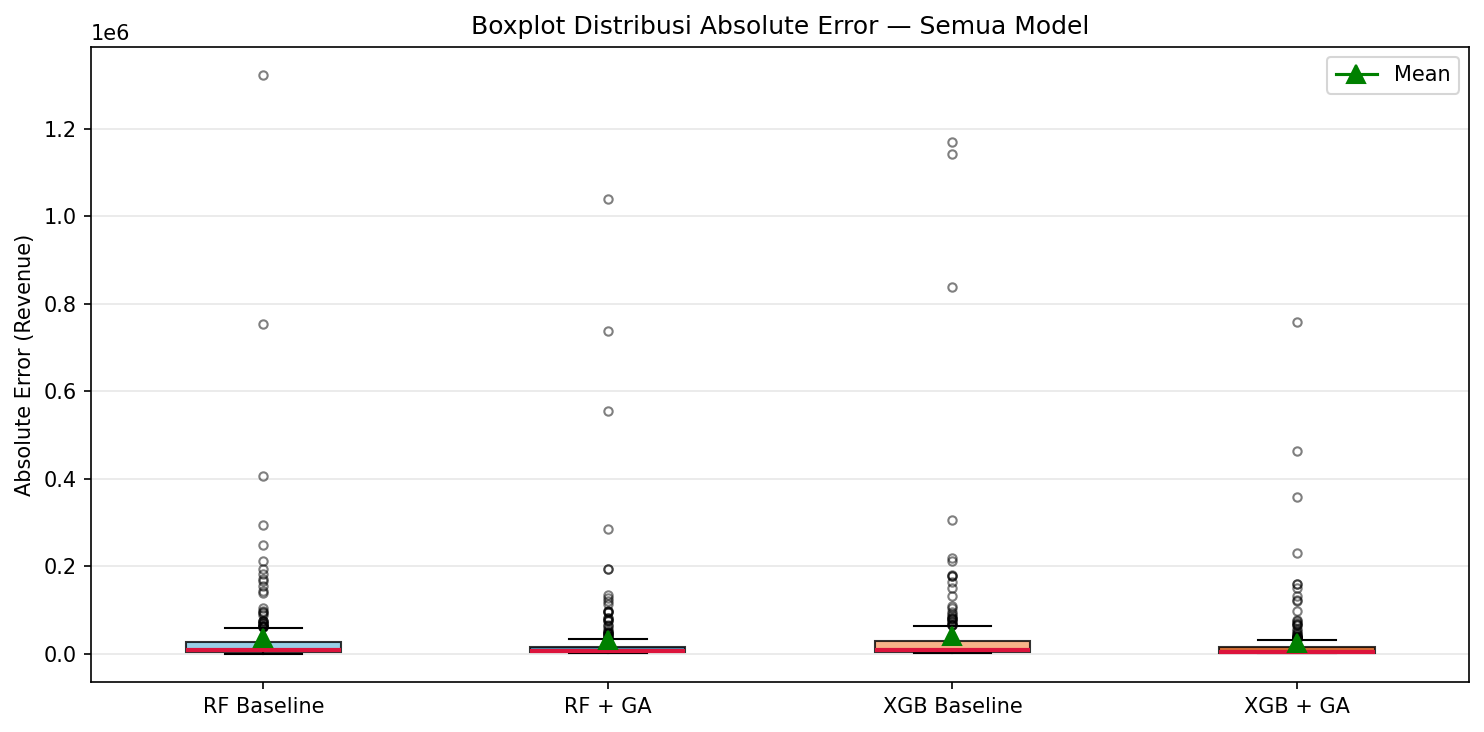
\includegraphics[width=0.7\textwidth]{tugas-akhir/assets/images/boxplot_error_models.png}
\caption{Perbandingan distribusi kesalahan prediksi (\textit{boxplot error}) keempat model}
\label{fig:boxplot_error}
\end{figure}

\begin{figure}[H]
\centering
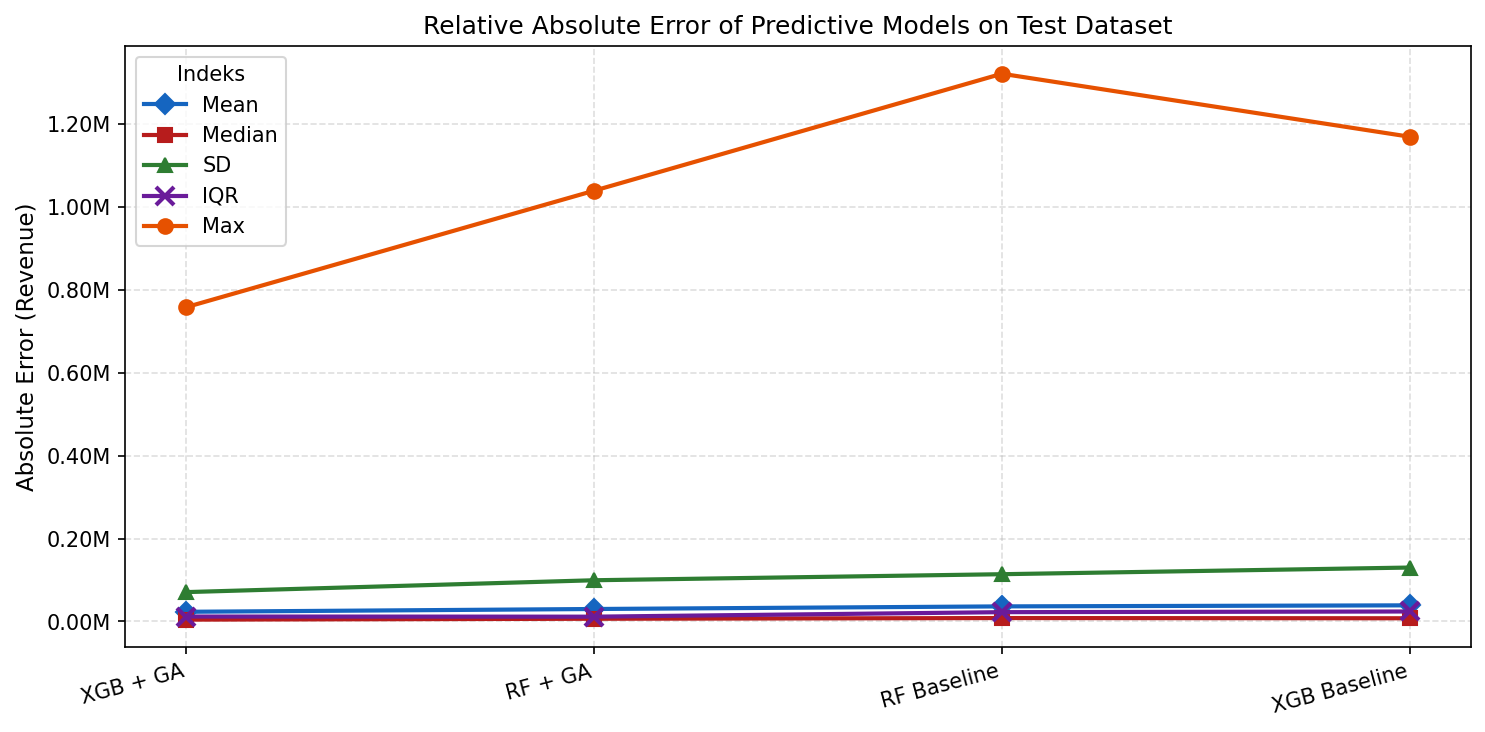
\includegraphics[width=0.7\textwidth]{tugas-akhir/assets/images/relative_absolute_error.png}
\caption{Indeks statistik deskriptif kesalahan prediksi seluruh model}
\label{fig:relative_absolute_error}
\end{figure}

Selain analisis kesalahan, kurva konvergensi GA ditunjukkan pada Gambar 4.10. Kurva ini memperlihatkan peningkatan nilai fungsi \textit{fitness} yang konsisten di setiap generasi untuk kedua model, mengkonfirmasi bahwa GA berhasil menavigasi ruang pencarian hiperparameter secara efektif. Konfigurasi hiperparameter optimal yang dihasilkan GA untuk masing-masing model ditunjukkan pada Tabel 4.10 dan Tabel 4.11.

\begin{figure}[H]
\centering
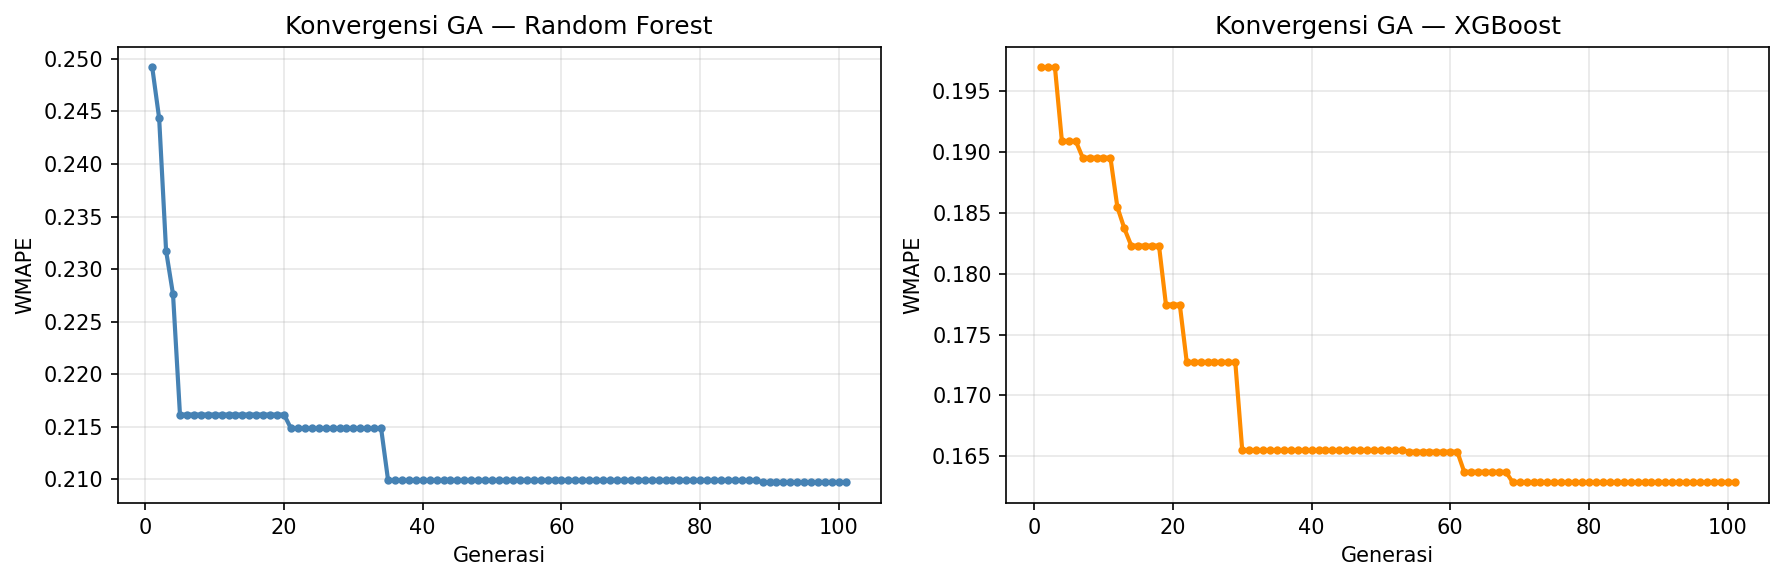
\includegraphics[width=0.92\textwidth]{tugas-akhir/assets/images/konvergensi_ga.png}
\caption{Kurva konvergensi fungsi \textit{fitness} GA untuk \textit{Random Forest} dan \textit{XGBoost}}
\label{fig:ga_convergence}
\end{figure}

\begin{table}[H]
\centering
\caption{Hiperparameter optimal \textit{Random Forest Regressor} hasil GA}
\label{tab:optimal_hp_rf}
\begin{tabular}{llc}
\toprule
\textbf{Hiperparameter} & \textbf{Ruang Pencarian} & \textbf{Nilai Optimal} \\
\midrule
\texttt{n\_estimators}       & [50, 1000]    & 68   \\
\texttt{max\_depth}          & [1, 7]         & 6     \\
\texttt{min\_samples\_split} & [2, 20]        & 6     \\
\texttt{min\_samples\_leaf}  & [1, 50]        & 2     \\
\texttt{max\_features}       & [1, 23]     & 8     \\
\texttt{max\_samples}        & [0{,}1, 1{,}0] & 0{,}393 \\
\bottomrule
\end{tabular}
\end{table}

\begin{table}[H]
\centering
\caption{Hiperparameter optimal \textit{XGBoost Regressor} hasil GA}
\label{tab:optimal_hp_xgb}
\begin{tabular}{llc}
\toprule
\textbf{Hiperparameter} & \textbf{Ruang Pencarian} & \textbf{Nilai Optimal} \\
\midrule
\texttt{learning\_rate}      & [0{,}001, 1{,}0]     & 0{.}0417 \\
\texttt{n\_estimators}       & [50, 1000]           & 182   \\
\texttt{max\_depth}          & [1, 7]                & 4     \\
\texttt{subsample}           & [0{,}1, 1{,}0]       & 0{,}546 \\
\texttt{colsample\_bytree}   & [0{,}1, 1{,}0]       & 0{,}977 \\
\texttt{reg\_lambda}         & [1, 3]                & 1{,}195 \\
\bottomrule
\end{tabular}
\end{table}


% \begin{table}[h]
% \centering
% \caption{Perbandingan Hasil Evaluasi Model Tahap Kedua}
% \label{tab:perbandingan_model}
% \begin{tabular}{llccc}
% \toprule
% \textbf{Model} & \textbf{Konfigurasi} & \textbf{WMAPE (\%)} & \textbf{$R^2$} & \textbf{MAE} \\
% \midrule
% Random Forest  & Baseline  & 24,82 & 0,9315 & 35\,485,88 \\
% Random Forest  & GA-Tuned  & 18,80 & 0,9717 & 26\,890,63 \\
% XGBoost        & Baseline  & 27,68 & 0,9207 & 39\,582,76 \\
% XGBoost        & GA-Tuned  & 15,46 & 0,9907 & 22\,107,41 \\
% \bottomrule
% \end{tabular}
% \end{table}

